\documentclass[a4paper, 12pt]{article}
\usepackage[a4paper,top=1.5cm, bottom=1.5cm, left=1cm, right=1cm]{geometry}

% Работа с русским языком
\usepackage[utf8]{inputenc}
\usepackage{mathtext}                % русские буквы в формулах
\usepackage[english, russian]{babel} % локализация и переносы

\usepackage{graphicx}   % Вставка изображений
\usepackage{float}      % "Плавающие" изображения3
\usepackage{wrapfig}    % Обтекание фигур (таблиц, картинок и прочего)
\usepackage{subfig}
\graphicspath{ {./images/} }

\usepackage{tabularx}
\usepackage{multirow}
\usepackage{amsmath}
\usepackage{amsfonts}
\usepackage{indentfirst}
\usepackage{longtable}
\graphicspath{{pictures/}}
\usepackage{natbib}
\usepackage{bm}

%%% Колонтитулы
\usepackage{titleps}
\newpagestyle{main}{
	\setheadrule{0.4pt}
	\sethead{Спектральный анализ электрических сигналов}{}{}
	\setfootrule{0.4pt}                       
	\setfoot{ФРКТ МФТИ, 2023}{}{\thepage} 
}
\pagestyle{main}  

\begin{document}
    \begin{titlepage}
	\begin{center}
            {\large МОСКОВСКИЙ ФИЗИКО-ТЕХНИЧЕСКИЙ ИНСТИТУТ (НАЦИОНАЛЬНЫЙ ИССЛЕДОВАТЕЛЬСКИЙ УНИВЕРСИТЕТ)}
	\end{center}
 
	\begin{center}
		{\large Физтех-школа радиотехники и компьютерных технологий}
	\end{center}
	
	\vspace{8cm}
	{\LARGE
		\begin{center}
                {\bf Отчёт о выполнении лабораторной работы 3.6.1}\\
                Спектральный анализ электрических сигналов
		\end{center}
	}
	\vspace{5cm}
	\begin{flushright}
		{\Large Автор:\\ Тихонов Дмитрий Романович, \\
			\vspace{0.2cm}
			студент группы Б01-206}
	\end{flushright}
	\vspace{5cm}
	\begin{center}
		\Large Долгопрудный, 2023
	\end{center}
    \end{titlepage}


    \section{Введение}

    \noindent \textbf{Цель работы:} изучить спектры сигналов различной формы и влияние параметров сигнала на вид соответствующих спектров; проверить справедливость соотношений неопределённостей; познакомиться с работой спектральных фильтров на примере RC-цепочки. \\

    \noindent \textbf{В работе используются:} генератор сигналов произвольной формы, цифровой осциллограф с функцией быстрого преобразования Фурье или цифровой USB-осциллограф, подключённый к персональному компьютеру.
    
    \section{Теоретические сведения}
    \label{theor}

    \subsection{Ряд Фурье и спектральный анализ}

    Согласно теореме Фурье, любая периодическая функция может быть представлена в виде ряда гармонических функций с кратными частотами — \textit{ряда Фурье}. Одно из представлений ряда Фурье для функции с периодом $T$ имеет вид

    \begin{equation}
        f(t) = \frac{A_0}{2} + \sum_{n=1}^{\infty} A_n \cos{(2\pi \nu_n t)} + B_n \sin{(2\pi \nu_n t)}, 
    \end{equation}

    где $\nu_n = n \nu_0$, $\nu_0 = \frac{1}{T}$, $n = 1,2, \cdots$ -- частоты фурье-гармоник, $A_n$ и $B_n$ — \textit{коэффициенты разложения} в ряд Фурье. Коэффициенты находятся как

    \begin{equation}
        A_n = \frac{2}{T} \int_{0}^T f(t) \cdot \cos{(2\pi \nu_n t)} dt, \hspace{4 mm} B_n = \frac{2}{T} \int_{0}^T f(t) \cdot \sin{(2\pi \nu_n t)} dt.
    \end{equation}

    Удобнее использовать эквивалентную форму записи ряда Фурье в \textit{представлении амплитуд и фаз}:

    \begin{equation}
        f(t) = \frac{a_0}{2} + \sum_{n=1}^{\infty} a_n \cos{(2\pi \nu_n t + \varphi_n)},
    \end{equation}

    где $a_n = \sqrt{A_n^2 + B_n^2}$ -- \textit{амплитуда} гармоники, а $\tg{\varphi_n} = B_n / A_n$ -- фаза.

    Совокупность всех частот $\nu_n$ и соответствующих им амплитуд $a_n$ и фаз $\varphi_n$ называют \textit{спектром функции} $f(t)$. Cпектр периодической функции \textit{дискретен} (число гармоник счётно). Если функция не периодическая, но ограниченная во времени, её можно представить как предел периодической функции с очень большим периодом $T \rightarrow \infty$. Тогда частотное расстояние между соседними гармониками $\delta \nu = 1/T$ стремится к нулю, то есть спектр становится \textit{непрерывным}. Разложение в ряд Фурье при этом переходит в \textit{интеграл Фурье}.

    Формулу (\ref{eq:dir_fourier}), в которой функции $f(t)$ ставится в соответствие функция $F(\omega)$ называют \textit{преобразованием Фурье}. Это преобразование является взаимно-однозначным, а восстановление исходной функции по её спектру называется \textit{обратным преобразованием Фурье}. Оно представлено формулой (\ref{eq:inv_fourier}).

    \begin{equation}
        F(\omega) = \int_{-\infty}^{\infty} f(t) e^{i \omega t} dt
        \label{eq:dir_fourier}
    \end{equation}

    \begin{equation}
        f(t) = \frac{1}{2\pi} \int_{-\infty}^{\infty} F(\omega) e^{i \omega t} d\omega
        \label{eq:inv_fourier}
    \end{equation}

    Однако при спектральном анализе электрических сигналов, как правило, измеряются именно амплитуды $\lvert a_n \rvert$ спектральных компонент, а информация об их фазах $\varphi_n$ теряется. Это приводит к тому, что пропадает взаимно-однозначное соответствие между сигналом и спектром, и весьма разные сигналы могут иметь один и тот же амплитудный спектр.

    \subsection{Периодическая последовательность прямоугольных импульсов}

    Найдём спектр периодической последовательности прямоугольных импульсов длительности $\tau$ с периодом следования импульсов $T > \tau$ (рис. \ref{impulse}).

    \begin{figure}[H]
        \centering
        \subfloat{{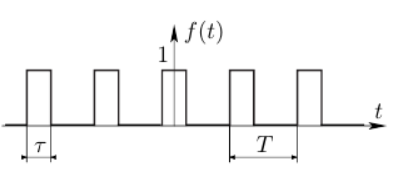
\includegraphics[width = 7 cm]{images/f(t)_impulse.png}}}
        \subfloat{{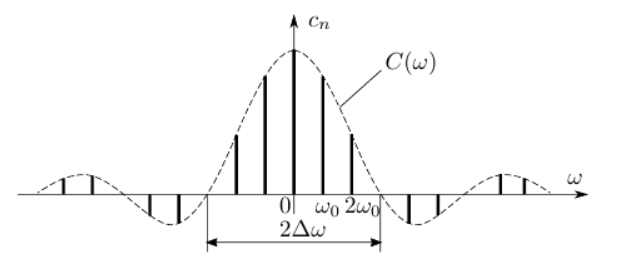
\includegraphics[width = 7 cm]{images/impulse_spectrum.png}}}
        \caption{Периодическая последовательность импульсов (слева) и её спектр (справа)}
        \label{impulse}
    \end{figure}

    \begin{equation}
        c_n = \frac{1}{T} \int_{-\tau/2}^{\tau/2} e^{-in \omega_0 t} dt = \frac{\tau}{T} \cdot \frac{\sin{(n\omega_0 \tau/2)}}{n\omega_0 \tau/2} = \frac{\sin{(\pi n \tau / T)}}{\pi n} = \frac{\tau}{T} \cdot \frac{\sin{(\pi \nu_n \tau)}}{\pi \nu_n \tau}.
        \label{eq:impulse}
    \end{equation}

    Спектр $\{c_n\}$ показан на рис. \ref{impulse}. Пунктирной кривой изображена огибающая функция

    \begin{equation}
        C(\omega) = \frac{\tau}{T} \cdot \frac{\sin{\omega \tau/2}}{\omega \tau/2}.
    \end{equation}

    Полуширина $\Delta \omega$ главного максимума этой функции определяется условием $\sin{\omega \tau/2} = 0$:

    \begin{equation*}
        \Delta \omega \cdot \frac{\tau}{2} = \pi \hspace{4 mm} \text{или} \hspace{4 mm} \Delta \omega \cdot \tau = 2\pi.
    \end{equation*}

    \subsection{Периодическая последовательность цугов}

    Найдём спектр обрывка синусоиды с частотой $\omega_0$ длительностью $\tau$ (такой сигнал называют \textit{цугом}). Сигнал может быть представлен как

    \begin{equation}
        f(t) = f_0(t) \cos{(\omega_0 t)},
    \end{equation}

    где $f_0(t)$ - единичный прямоугольный импульс длительностью $\tau$ (рис. \ref{zug_f(t)}).

    \begin{figure}[H]
        \centering
        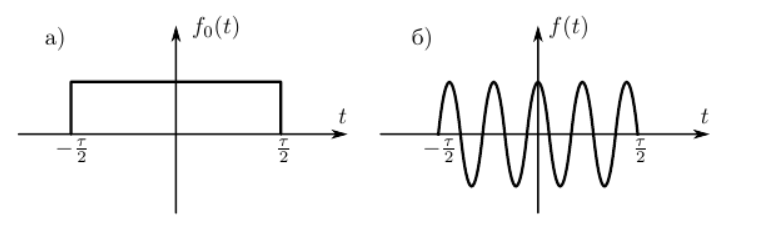
\includegraphics[width = 14 cm]{images/zug_f(t).png}
        \caption{Прямоугольный (а) и синусоидальный (б) импульсы}
        \label{zug_f(t)}
    \end{figure}

    Найдём спектр прямоугольного импульса длительности $\tau$ единичной амплитуды:

    \begin{equation}
        F_0(\omega) = \int_{-\tau/2}^{\tau/2} e^{-i \omega t} dt = \tau \frac{\sin{\omega \tau /2}}{\omega \tau /2}.
    \end{equation}

    Соотношение для смещения спектра:

    \begin{equation}
        F(\omega) = \frac{1}{2} F_0(\omega - \omega_0) + \frac{1}{2} F_0(\omega + \omega_0).
    \end{equation}

    Отсюда, получим

    \begin{equation}
        F(\omega) = \frac{\tau}{2} \left[\frac{\sin{(\omega - \omega_0) \tau/2}}{(\omega - \omega_0) \tau/2} + \frac{\sin{(\omega + \omega_0) \tau/2}}{(\omega + \omega_0) \tau/2}\right].
    \end{equation}

    Спектры $F_0(\omega)$ и $F(\omega)$ представлены на рис. \ref{spectrum_zug}.

    \begin{figure}[H]
        \centering
        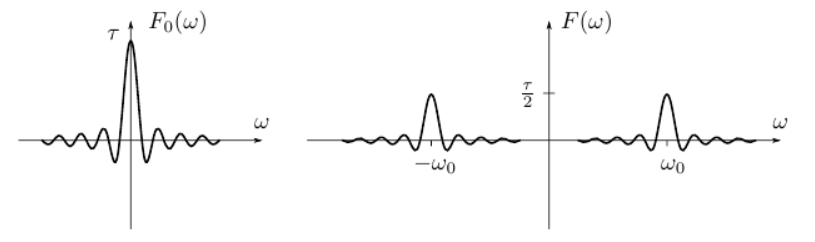
\includegraphics[width = 14 cm]{images/zug_F(omega).png}
        \caption{Спектры прямоугольного импульса и синусоидального цуга}
        \label{spectrum_zug}
    \end{figure}

    Сравнивая спектр последовательности прямоугольных импульсов и цугов мы видим, что они аналогичны, но их максимумы сдвинуты по частоте на величину $\omega_{0}$.

    \subsection{Соотношения неопределённсотей}

    \label{theor_uncertainty}

    Если у сигнала $f(t)$ есть какое характерное время $\Delta t$, то в спектре $a(\nu)$ будет наблюдаться характерный масштаб $\Delta \nu \sim 1/\Delta t$. Соотношения вида

    \begin{equation}
        \Delta \nu \cdot \Delta t \sim 1
    \end{equation}

    принято называть \textit{соотношениями неопределённостей}.

    Например, если $\Delta t = \tau$ — характерная \textit{длительность} импульса, то характерная \textit{ширина} спектра по порядку величины будет равна $\Delta \nu \sim 1/\tau$. Конкретное числовое значение зависит, во-первых, от детальной формы сигнала, и, во-вторых, от того, что именно мы называем \textit{характерным} временем и что — \textit{шириной} спектра.
    
    Другой пример, для любого сигнала с периодом $T$ в спектре обязательно будут наблюдаться гармоники на расстоянии $\delta \nu = 1/T$ друг от друга. В данном случае соотношение является точным и от формы сигнала не зависит.

    \subsection{Амплитудная модуляция}

    Рассмотрим простейшее амплитудно-модулированное колебание, в котором амплитуда модуляции является гармонической функцией:

    \begin{equation}
        f(t) = a(t) \cos{(\omega_0 t)} = a_0 (1 + m \cos{\Omega t}) \cos{\omega_0 t} = a_0 \cos{\omega_0 t} + \frac{ma_0}{2} \cos{(\omega_0 + \Omega) t} + \frac{ma_0}{2} \cos{(\omega_0 - \Omega) t} .
        \label{eq:modulation_f(t)_1}
    \end{equation}

    Итак, амплитудно-модулированное колебание представляется в виде суммы трёх гармонических колебаний:

    \begin{equation}
        f_0(t) = a_0 \cos{\omega_0 t}, \hspace{1 mm} f_1(t) = \frac{ma_0}{2} \cos{(\omega_0 + \Omega) t}, \hspace{1 mm} f_2(t) = \frac{ma_0}{2} \cos{(\omega_0 - \Omega) t}
    \end{equation}

    с частотами соответственно $\omega_0$, $\omega_0 + \Omega$, $\omega_0 - \Omega$ и амплитудами $a_0$, $ma_0/2$, $ma_0/2$. Колебание $f_0(t)$ называется \textit{несущим колебанием}, а $f_1(t)$ и $f_2(t)$ -- \textit{боковыми гармониками}.

    Константа $0 < m \leq 1$ называется \textit{глубиной модуляции}. Глубину модуляции можно выразить через максимальную $a_{max}$ и минимальную $a_{min}$ амплитуды сигнала:

    \begin{equation}
        m = \frac{a_{max} - a_{min}}{a_{max} + a_{min}}.
    \end{equation}

    \subsection{Интегрирующая \textit{RC}-цепочка}

     \begin{wrapfigure}{l}{4cm}
        \centering
	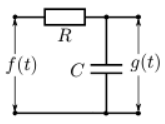
\includegraphics[width=3cm]{images/int_RC.png}
	\caption{Интегрирующая \textit{RC}-цепочка}
	\label{int_RC}
    \end{wrapfigure}

    Частотная характеристика \textit{RC}-цепочки (рис. \ref{int_RC}) равна

    \begin{equation}
        \lambda(\omega) = \frac{1}{1 + i \omega \tau_{RC}}.
    \end{equation}

    Отсюда, амплитудный коэффициент фильтрации равен

    \begin{equation}
        K(\nu) = \frac{1}{\sqrt{1 + 4\pi^2 \nu^2 R^2 C^2}}
    \end{equation}\\

    При $2\pi \nu \gg 1/\tau_{RC}$ имеем $K \approx \frac{1}{2 \pi \nu RC} \rightarrow 0$, то есть \textit{RC}-цепочка подавляет все компоненты сигнала с достаточно высокой частотой, а низкочастотные компоненты пропускает без искажения ($K \rightarrow 1$ при $2\pi \nu \ll 1/\tau_{RC} $). Такие устройства называют \textit{фильтрами низких частот}.
    
    \section{Методика измерений и используемое оборудование}

    Вследствие того, что частота исследуемого сигнала не слишком велика (заведомо меньше тактовой частоты процессоров), в данной работе применяется цифровой спектральный анализ, который имеет две отличительные особенности.

    Во-первых, при цифровом анализе возникает \textit{частота дискретизации} $\nu_\text{дискр}$, то есть частота, с которой считываются значения напряжения, подаваемого на входной канал анализатора. Дискретизация не позволит исследовать спектр частот, превышающих частоту $\nu_\text{дискр}$, и исказит спектр вблизи неё, поэтому надёжно получать спектр можно лишь на достаточно низких частотах $\nu \ll \nu_\text{дискр}$. Внутренняя частота дискретизации осциллографов обычно велика (типичное значение — $1$ ГГц), однако для преобразования Фурье в целях оптимизации скорости работы она может существенно урезаться. В настройках цифровых осциллографов часто используется параметр \textit{количество точек» на интервал времени}. Например, если сигнал записывался в течение $1$ с, то при стандартных для многих осциллографов $4096$ точках дискретизации,спектр будет заведомо ограничен лишь частотой $\sim 2$ кГц.
    
    Во-вторых, интервал времени $\Delta t$, в течение которого регистрируется сигнал, всегда ограничен. Для анализа сигнала вырезается его участок — \textit{окно} $t \in [t_0; t_0 + \Delta t]$. Такое преобразование Фурье часто называют \textit{оконным}. Из-за ограниченности размеров \textit{окна} неизбежно возникают дополнительные искажения спектра. Чтобы компенсировать эти искажения, значениям регистрируемой функции в пределах \textit{окна} придают разный вес. В таком случае говорят об \textit{оконной} функции преобразования Фурье. На практике применяются различные оконные функции, каждая из которых обладает своими достоинствами и недостатками (одни уменьшают шумы, другие уменьшают ширину пиков и погрешность частоты, третьи погрешность измерения амплитуд и т.д.). В нашей работе важно аккуратное измерения амплитуд, для чего лучше всего подходят окна \textit{окна с плоской вершиной}.

    \section{Результаты измерений и обработка данных}

    \subsection{Исследование спектра периодической последовательности прямоугольных импульсов и проверка соотношений неопределённостей}

    Настроив генерацию прямоугольных импульсов с частотой повторения $\nu_\text{повт} = 1$ кГц (период $T = 1$ мс) и длительностью импульса $\tau = T/20 = 50$  мкс, получили на экране спектр сигнала. Изменяя на генераторе параметры сигнала, зафиксировали, как изменялся спектр (рис. \ref{spectrum_A}).

    При фиксированных параметрах $\nu_\text{повт} = 1$ кГц и $\tau = 50$ мкс, были измерены амплитуды $a_n$ и частоты $\nu_n$ нескольких спектральных компонент (\textit{гармоник}). Результаты измерений представлены в таблице \ref{harmonic_relations}. 

    \begin{table}[H]
        \centering
        \begin{tabular}{|c|c|c|c|c|c|}
        \hline
        $n$ & $\nu_{n}^{exp}$, Гц & $\nu_{n}^{theor}$, Гц & $\lvert a_n\rvert^{exp}$, усл. ед. & $\lvert a_n/a_1\rvert^{exp}$ & $\lvert a_n/a_1\rvert^{theor}$ \\ \hline
        1 & 1021 & 1000 & 284,6 & 1,000 & 1,000 \\ \hline
        2 & 2045 & 2000 & 280,3 & 0,985 & 0,988 \\ \hline
        3 & 2994 & 3000 & 273,7 & 0,962 & 0,967 \\ \hline
        4 & 4056 & 4000 & 266,5 & 0,936 & 0,939 \\ \hline
        5 & 5042 & 5000 & 256,4 & 0,901 & 0,904 \\ \hline
        6 & 6028 & 6000 & 244,0 & 0,857 & 0,862 \\ \hline
        7 & 7014 & 7000 & 231,0 & 0,812 & 0,814 \\ \hline
        8 & 8001 & 8000 & 214,4 & 0,753 & 0,760 \\ \hline
        9 & 9025 & 9000 & 199,1 & 0,700 & 0,702 \\ \hline
        10 & 10001 & 10000 & 180,3 & 0,634 & 0,639 \\ \hline
        11 & 11040 & 11000 & 161,5 & 0,567 & 0,574 \\ \hline
        12 & 12020 & 12000 & 143,4 & 0,504 & 0,507 \\ \hline
        \end{tabular}
        \caption{Результаты исследования амплитуд и частот гармоник}
        \label{harmonic_relations}
    \end{table}

    При составлении таблицы были использованы соотношения \ref{eq:impulse}.

    Зафиксировав период повторения $T = 1$ мс прямоугольного сигнала, исследуем зависимость полной ширины спектра сигнала $\Delta \nu$ от длительности импульса $\tau$. Результаты измерений представлены в таблице \ref{nu_tau}.

    По этим данным построим график зависимости $\Delta \nu \left( 1/\tau \right)$ (рис. \ref{graph:nu_tau}).

    \begin{table}[H]
        \centering
        \begin{tabular}{|c|c|c|}
        \hline
        $\tau$, мкс & $\Delta \nu$, кГц & $1/\tau$, $10^3 \cdot \text{с}^{-1}$  \\ \hline
        50 & 19,6 & 20 \\ \hline
        75 & 13,4 & 13 \\ \hline
        100 & 9,8 & 10 \\ \hline
        125 & 8,0 & 8 \\ \hline
        150 & 6,5 & 7 \\ \hline
        175 & 5,5 & 6 \\ \hline
        200 & 4,5 & 5 \\ \hline
        \end{tabular}
        \caption{Результаты измерения зависимости $\Delta \nu$ от $\tau$}
        \label{nu_tau}
    \end{table}

    \begin{figure}[H]
        \centering
        \subfloat[$\nu_{\text{повт}} = 1,0$ кГц, $\tau = 50$ мкс]{{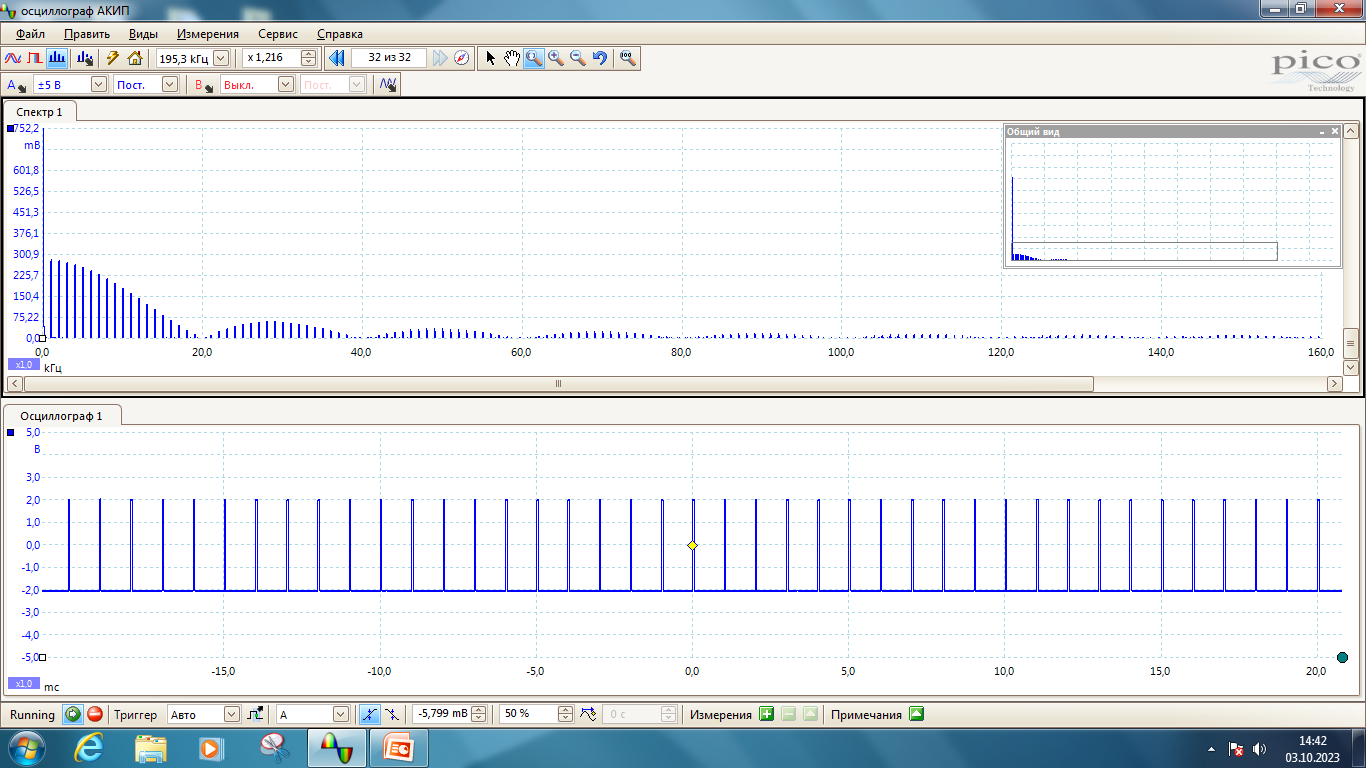
\includegraphics[width = 0.5\textwidth]{images/spectrum_A_1.png}}}
        \subfloat[$\nu_{\text{повт}} = 2,0$ кГц, $\tau = 50$ мкс]{{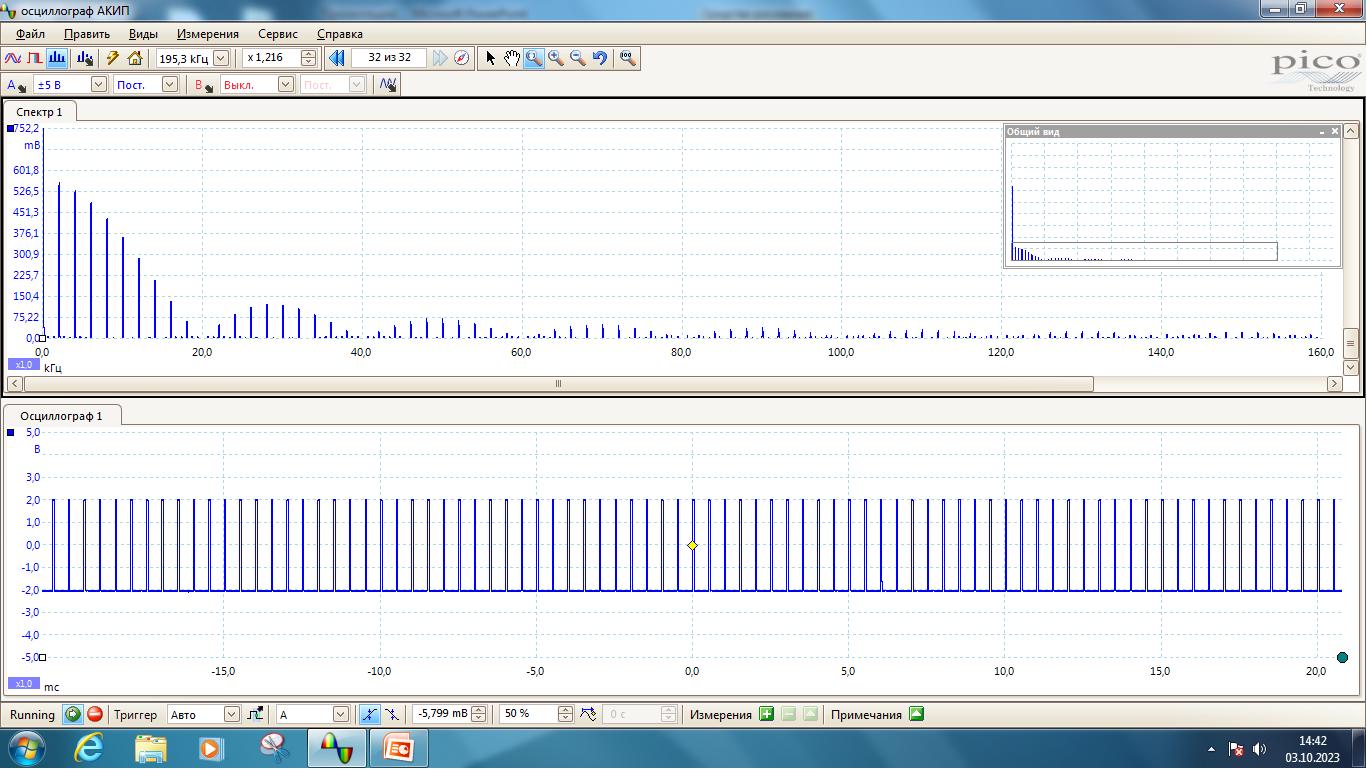
\includegraphics[width = 0.5\textwidth]{images/spectrum_A_2.png}}} \\
        \subfloat[$\nu_{\text{повт}} = 1,5$ кГц, $\tau = 50$ мкс]{{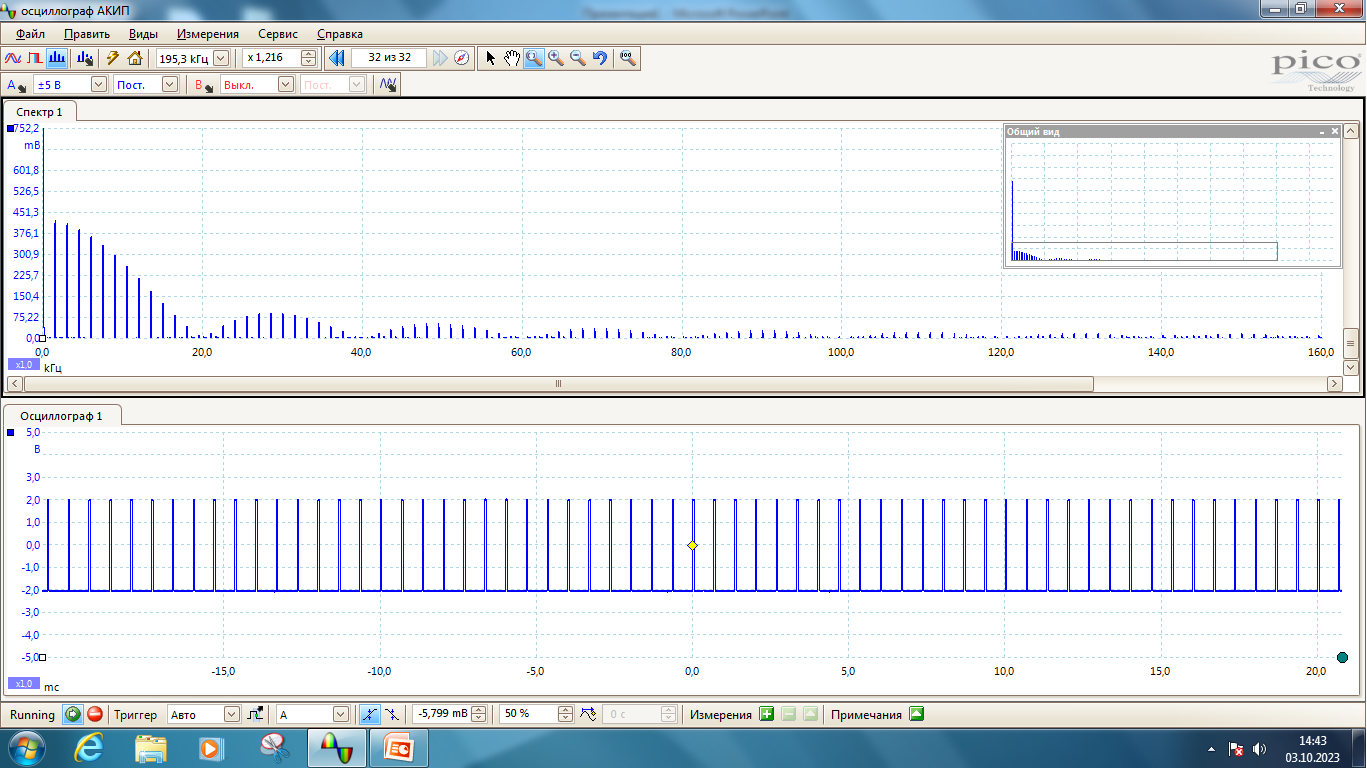
\includegraphics[width = 0.5\textwidth]{images/spectrum_A_3.png}}}
        \subfloat[$\nu_{\text{повт}} = 0,5$ кГц, $\tau = 50$ мкс]{{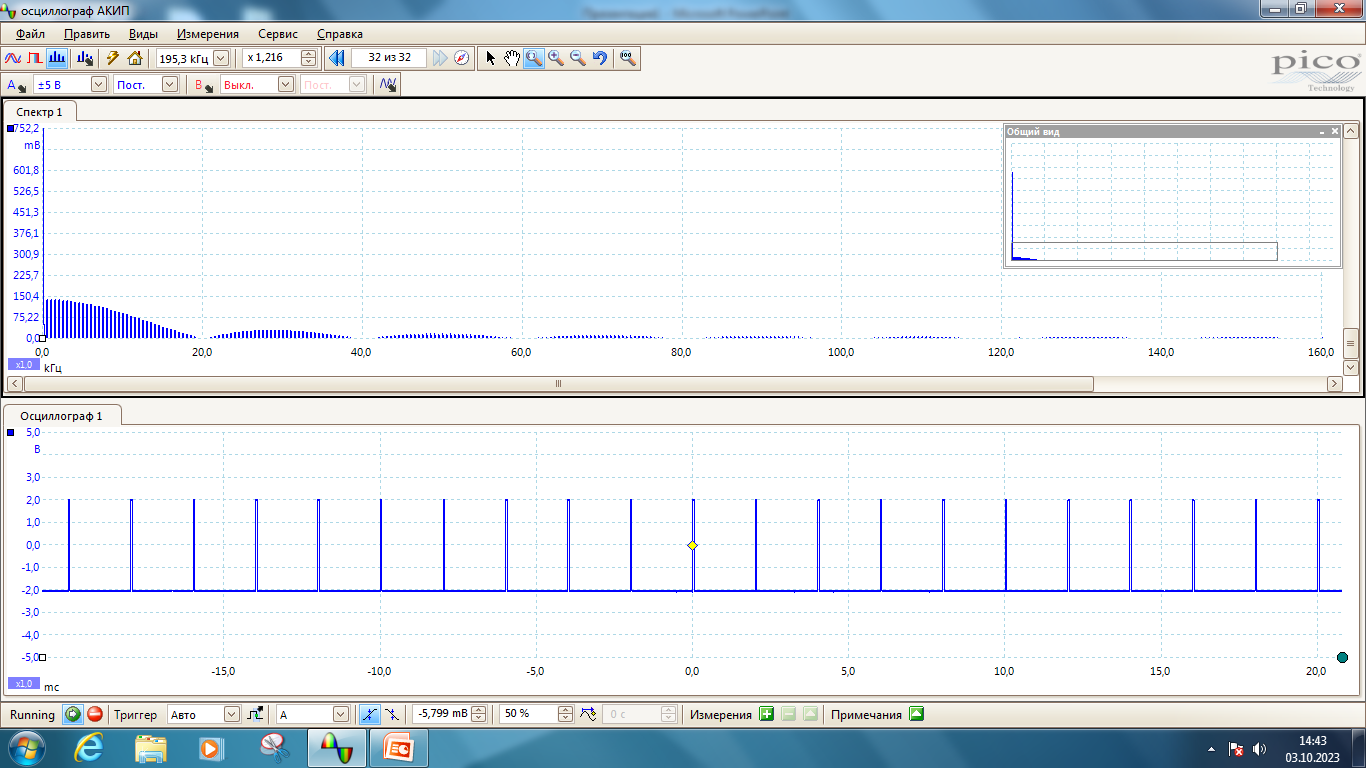
\includegraphics[width = 0.5\textwidth]{images/spectrum_A_4.png}}} \\
        \subfloat[$\nu_{\text{повт}} = 1,0$ кГц, $\tau = 60$ мкс]{{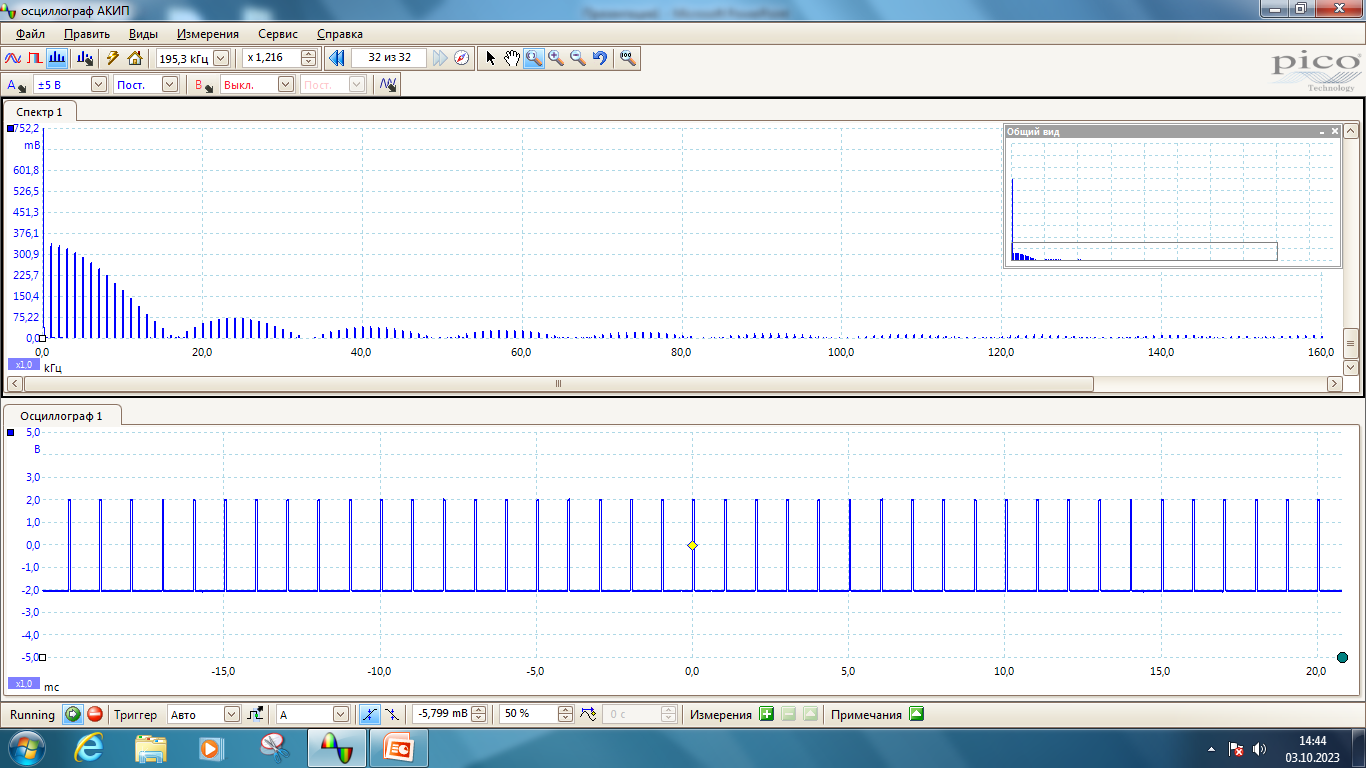
\includegraphics[width = 0.5\textwidth]{images/spectrum_A_5.png}}}
        \subfloat[$\nu_{\text{повт}} = 1,0$ кГц, $\tau = 70$ мкс]{{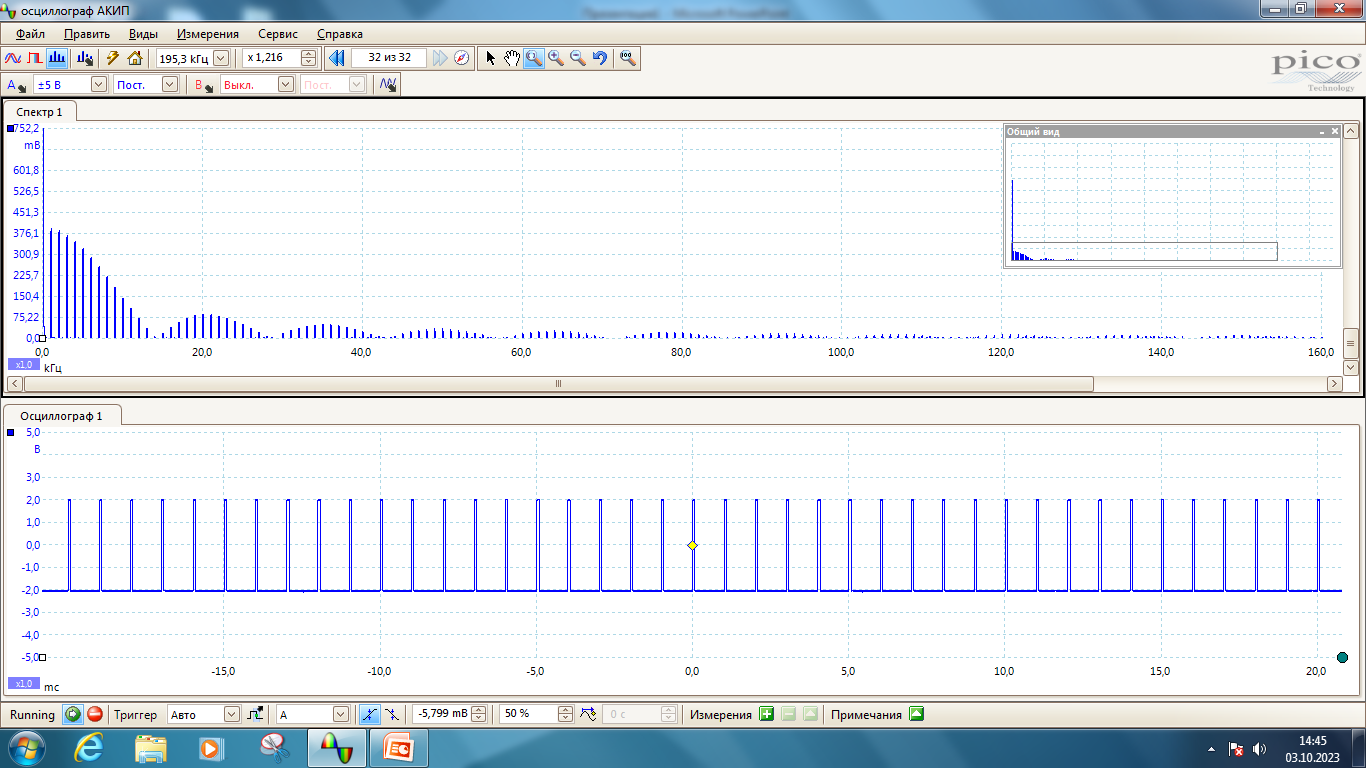
\includegraphics[width = 0.5\textwidth]{images/spectrum_A_6.png}}} \\
        \subfloat[$\nu_{\text{повт}} = 1,0$ кГц, $\tau = 90$ мкс]{{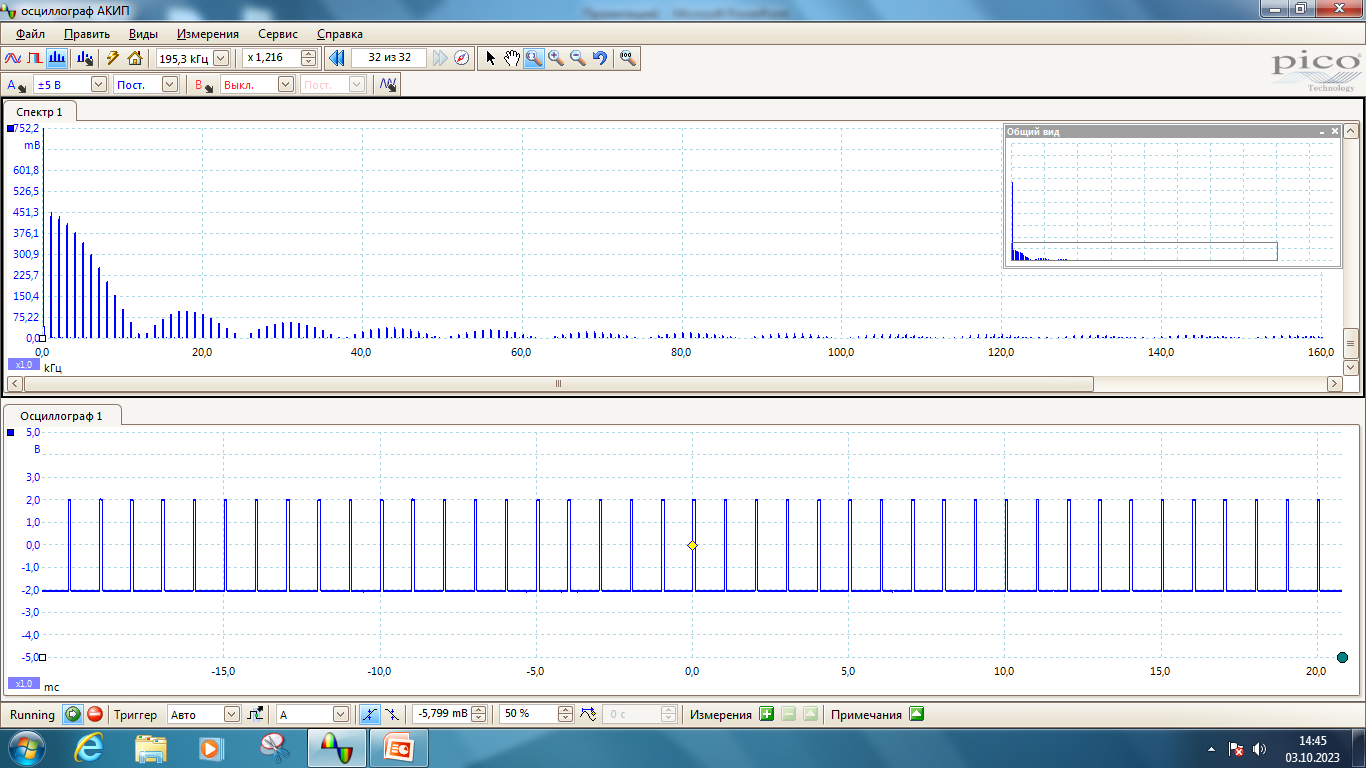
\includegraphics[width = 0.5\textwidth]{images/spectrum_A_7.png}}}
        \caption{Изменение спектра прямоугольных импульсов при варьировании параметров}
        \label{spectrum_A}
    \end{figure} 

    \begin{figure}[H]
        \centering
        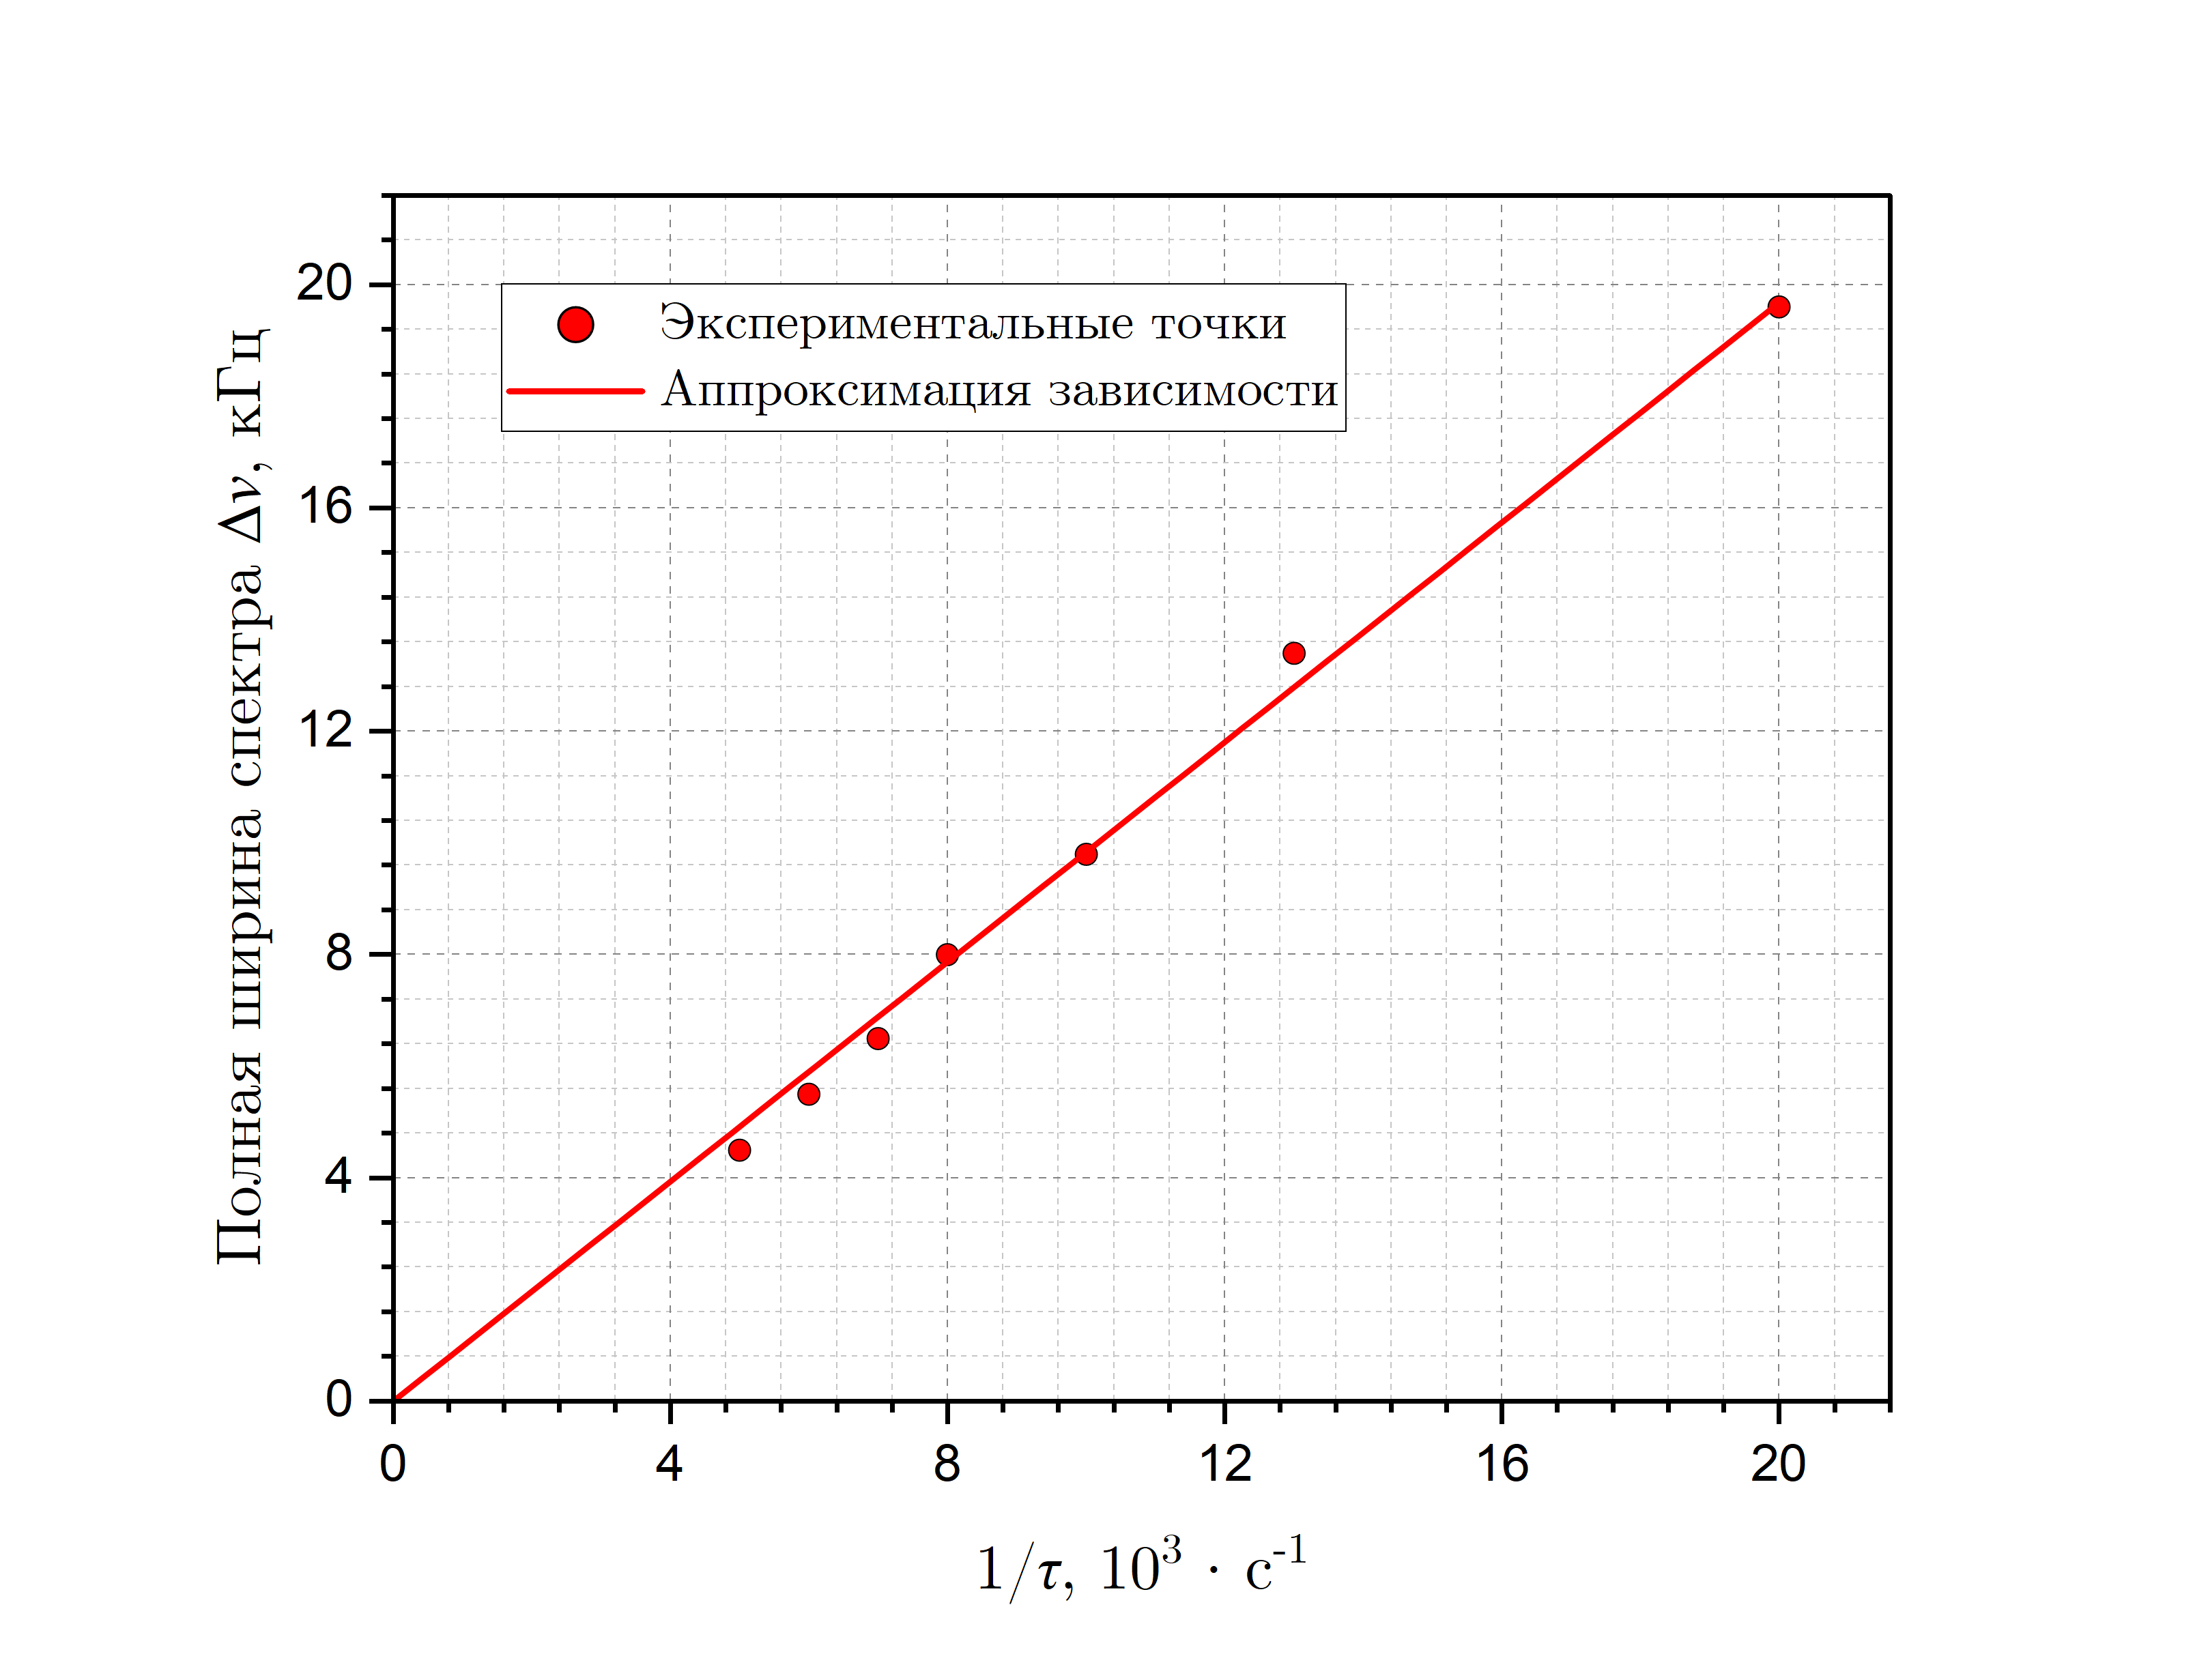
\includegraphics[width = 14 cm]{images/graph_nu_tau.png}
        \caption{График зависимости полной ширины спектра $\Delta \nu$ от $1/\tau$}
        \label{graph:nu_tau}
    \end{figure}

    Аппроксимируя полученные данные при помощи программы \textit{OriginPro 2023b}, получим

    $$
    \boxed{\Delta \nu \cdot \tau = 0,99 \pm 0,01 \sim 1}, 
    $$

    что согласуется с соотношением неопределённости (см. пункт \ref{theor_uncertainty}).

    Зафиксировав период повторения $\tau = 100$ мкс прямоугольного сигнала, исследуем зависимость расстояния $\delta \nu$ между соседними гармониками спектра от периода повторения $T$. Результаты измерений представлены в таблице \ref{nu_T}.

    \begin{table}[H]
        \centering
        \begin{tabular}{|c|c|c|}
        \hline
        $T$, мc & $\delta \nu$, кГц & $1/T$, $10^{3} \cdot \text{с}^{-1}$ \\ \hline
        0,2 & 5,000 & 5,000 \\ \hline
        1,0 & 1,014 & 1,000 \\ \hline
        1,8 & 0,554 & 0,556 \\ \hline
        2,6 & 0,374 & 0,385 \\ \hline
        3,4 & 0,307 & 0,294 \\ \hline
        4,2 & 0,241 & 0,238 \\ \hline
        5,0 & 0,203 & 0,200 \\ \hline
        \end{tabular}
        \caption{Результаты измерения зависимости $\delta \nu$ от $T$}
        \label{nu_T}
    \end{table}

    По этим данным построим график зависимости $\delta \nu \left( 1/T \right)$ (рис. \ref{graph:nu_T}).

    \begin{figure}[H]
        \centering
        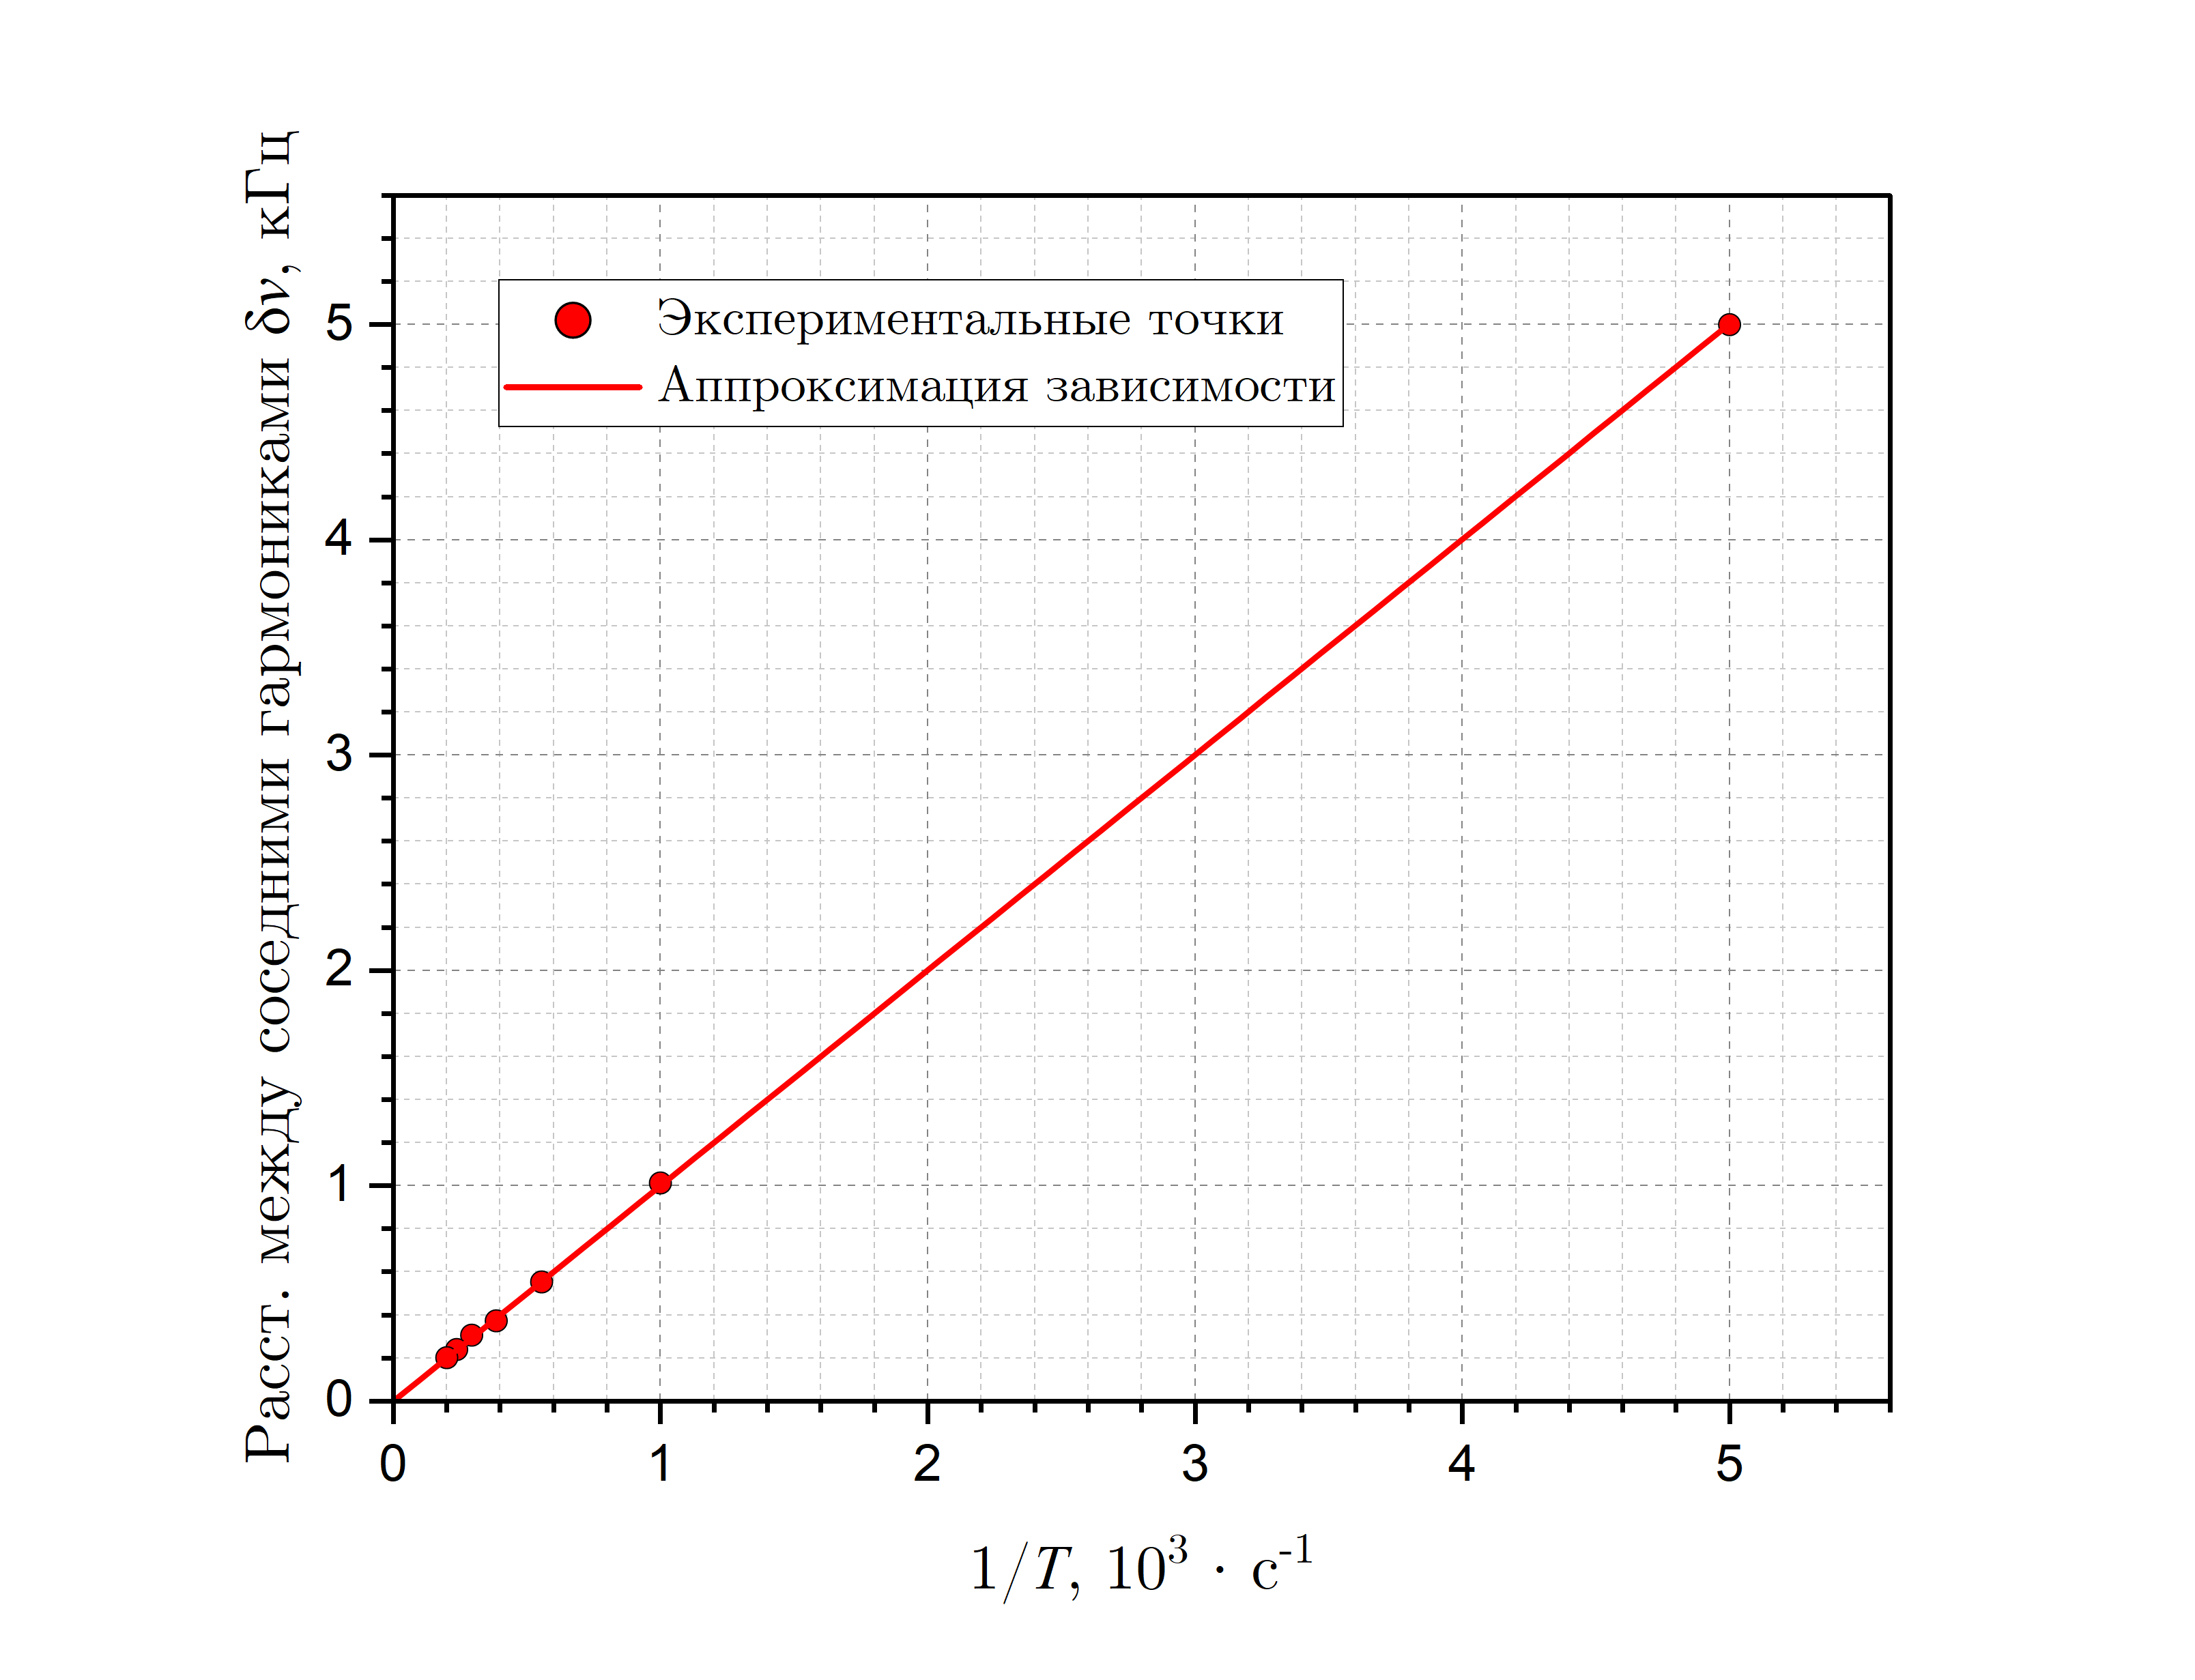
\includegraphics[width = 14 cm]{images/graph_nu_T.png}
        \caption{График зависимости расстояния между соседними гармониками $\delta \nu$ от $1/T$}
        \label{graph:nu_T}
    \end{figure}

    Аппроксимируя полученные данные при помощи программы \textit{OriginPro 2023b}, получим

    $$
    \boxed{\delta \nu \cdot T = 1,000 \pm 0,001}, 
    $$

    что согласуется с соотношением неопределённости (см. пункт \ref{theor_uncertainty}).

    \subsection{Наблюдение спектра периодической последовательности цугов}

    Настроив генерацию периодических импульсов синусоидальной формы (\textit{цугов}) с несущей частотой $\nu_0 = 50$ кГц, периодом повторения $T = 1$ мс ($\nu_\text{повт} = 1$ кГц) и числом периодов синусоиды в одном импульсе $N = 5$, получили на экране осциллографа устойчивую картину сигнала. Изменяя на генераторе параметры сигнала, зафиксировали, как изменялся спектр (рис. \ref{spectrum_B}).

    Теперь установим на генераторе следующие параметры: $\nu_0 = 50$ кГц, $N = 5$, для них измерим, меняя $T$, зависимость $\delta \nu$ от $1/T$. Полученные результаты исследования зависимости приведены в таблице \ref{table:zug}.

    \begin{table}[H]
        \centering
        \begin{tabular}{|c|c|c|c|}
        \hline
        $T$, мс & $\Delta \nu$, кГц & $\delta \nu$, кГц & $1/T$, $10^{3} \cdot \text{с}^{-1}$ \\ \hline
        4,00 & 10 & 0,25 & 0,25 \\ \hline
        2,00 & 10 & 0,55 & 0,50 \\ \hline
        1,00 & 10 & 0,97 & 1,00 \\ \hline
        0,50 & 10 & 1,94 & 2,00 \\ \hline
        0,25 & 10 & 4,00 & 4,00 \\ \hline
        0,20 & 10 & 5,00 & 5,00 \\ \hline
        \end{tabular}
        \caption{Результаты измерения зависимости $\delta \nu$ от $1/T$}
        \label{table:zug}
    \end{table}

    \begin{figure}[H]
        \centering
        \subfloat[$\nu_0 = 50$ кГц, $T = 1$ мс, $N = 5$]{{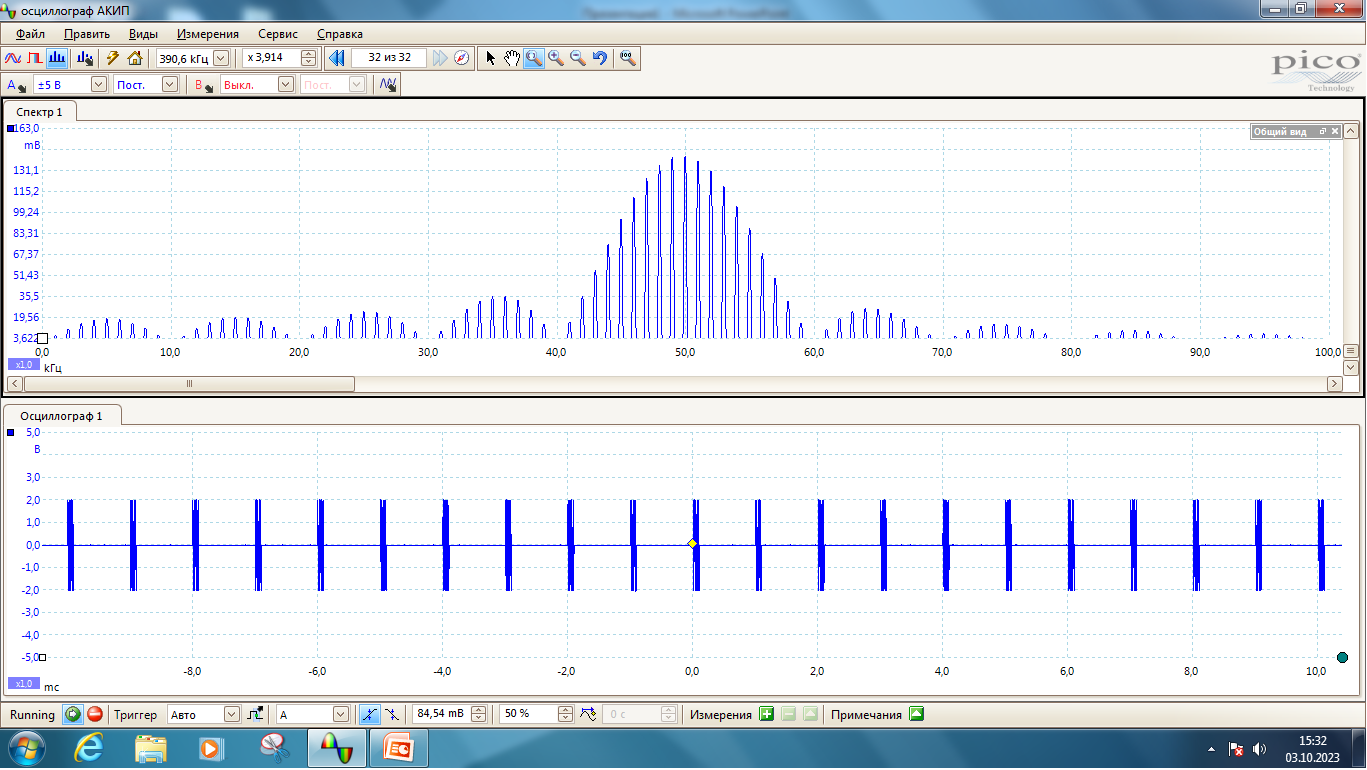
\includegraphics[width=0.5\textwidth]{images/spectrum_B_1.png}}}
        \subfloat[$\nu_0 = 50$ кГц, $T = 2$ мс, $N = 5$]{{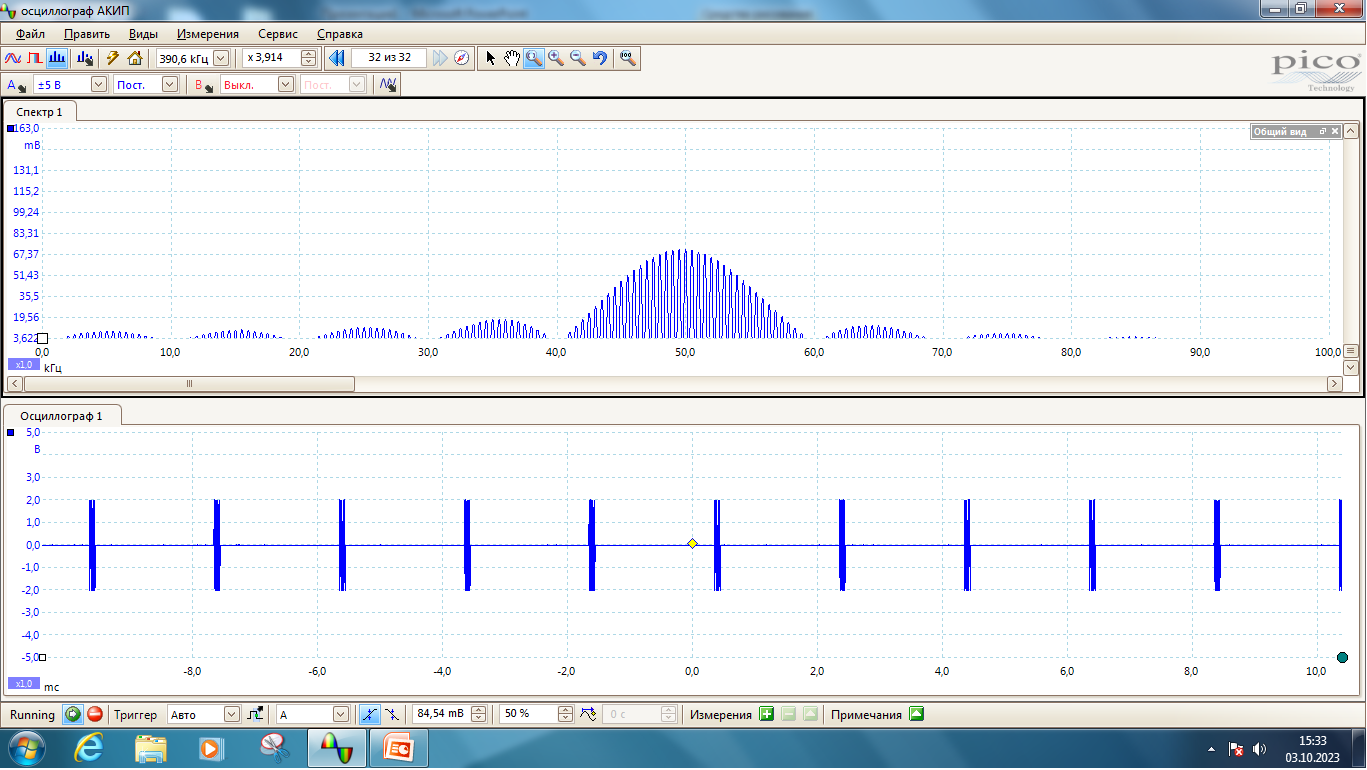
\includegraphics[width=0.5\textwidth]{images/spectrum_B_2.png}}} \\
        \subfloat[$\nu_0 = 50$ кГц, $T = 3$ мс, $N = 5$]{{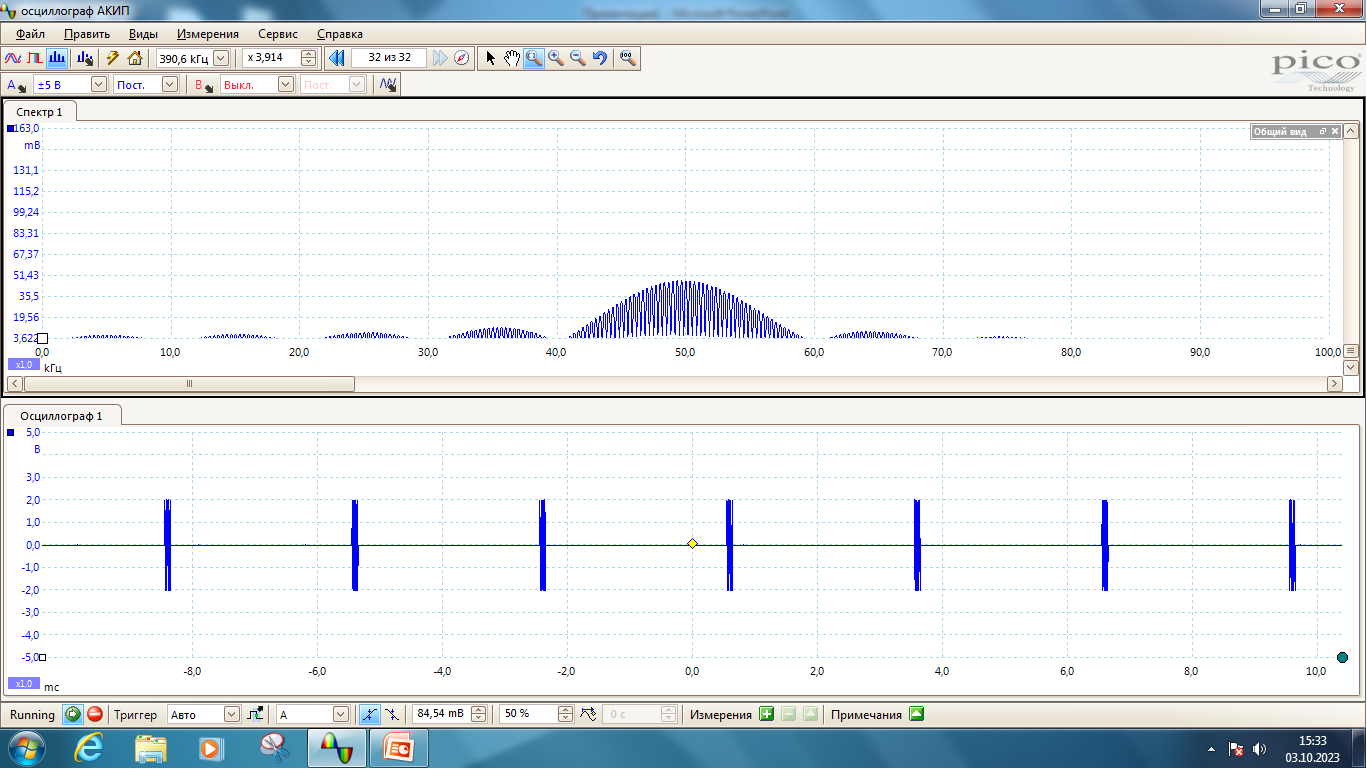
\includegraphics[width=0.5\textwidth]{images/spectrum_B_3.png}}}
        \subfloat[$\nu_0 = 50$ кГц, $T = 1$ мс, $N = 4$]{{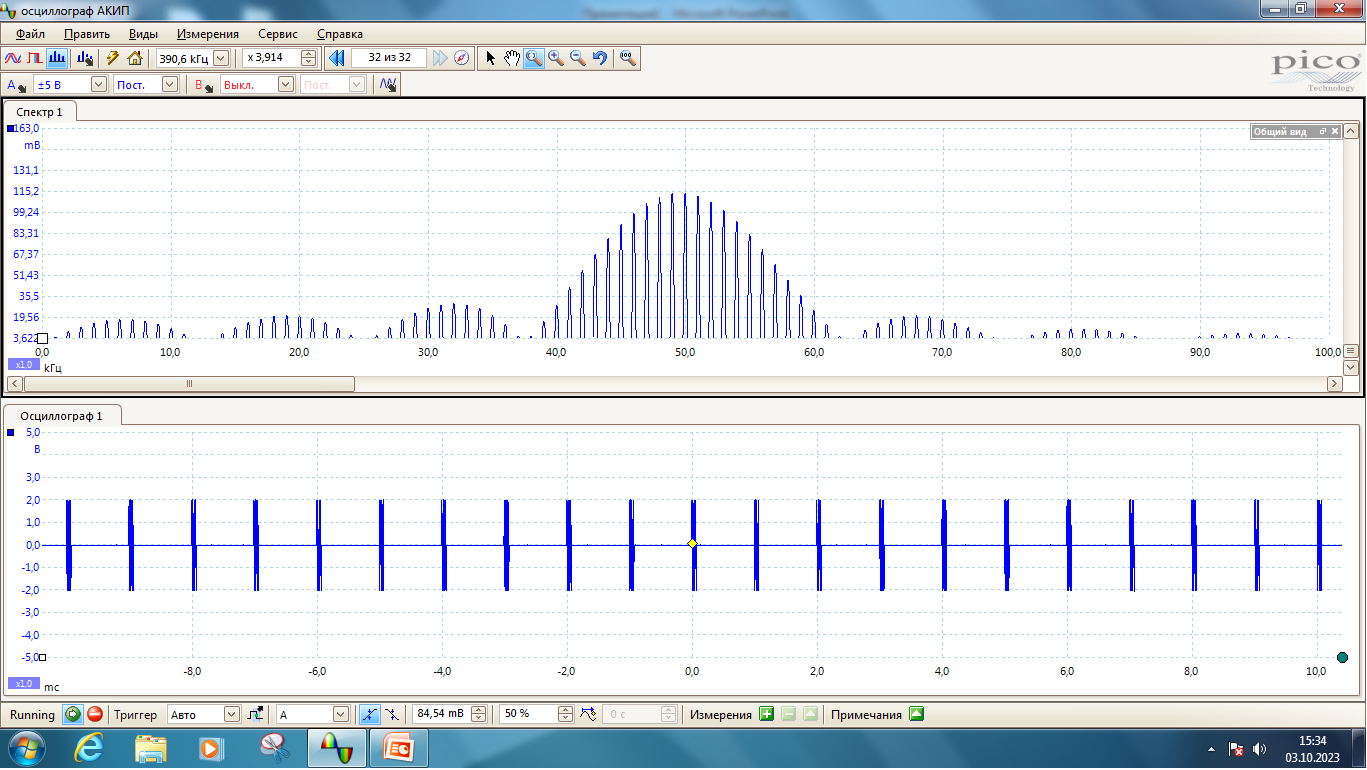
\includegraphics[width=0.5\textwidth]{images/spectrum_B_4.png}}} \\
        \subfloat[$\nu_0 = 50$ кГц, $T = 1$ мс, $N = 6$]{{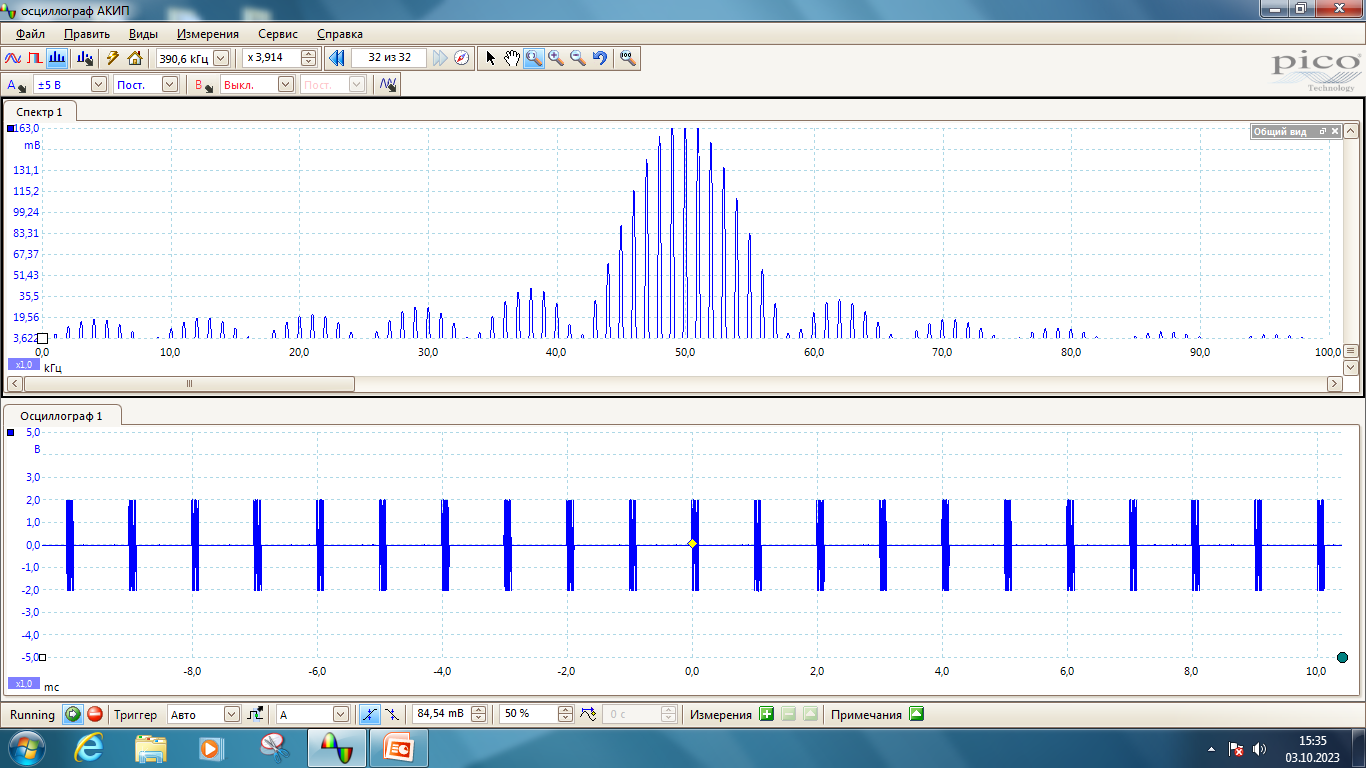
\includegraphics[width=0.5\textwidth]{images/spectrum_B_5.png}}}
        \subfloat[$\nu_0 = 60$ кГц, $T = 1$ мс, $N = 5$]{{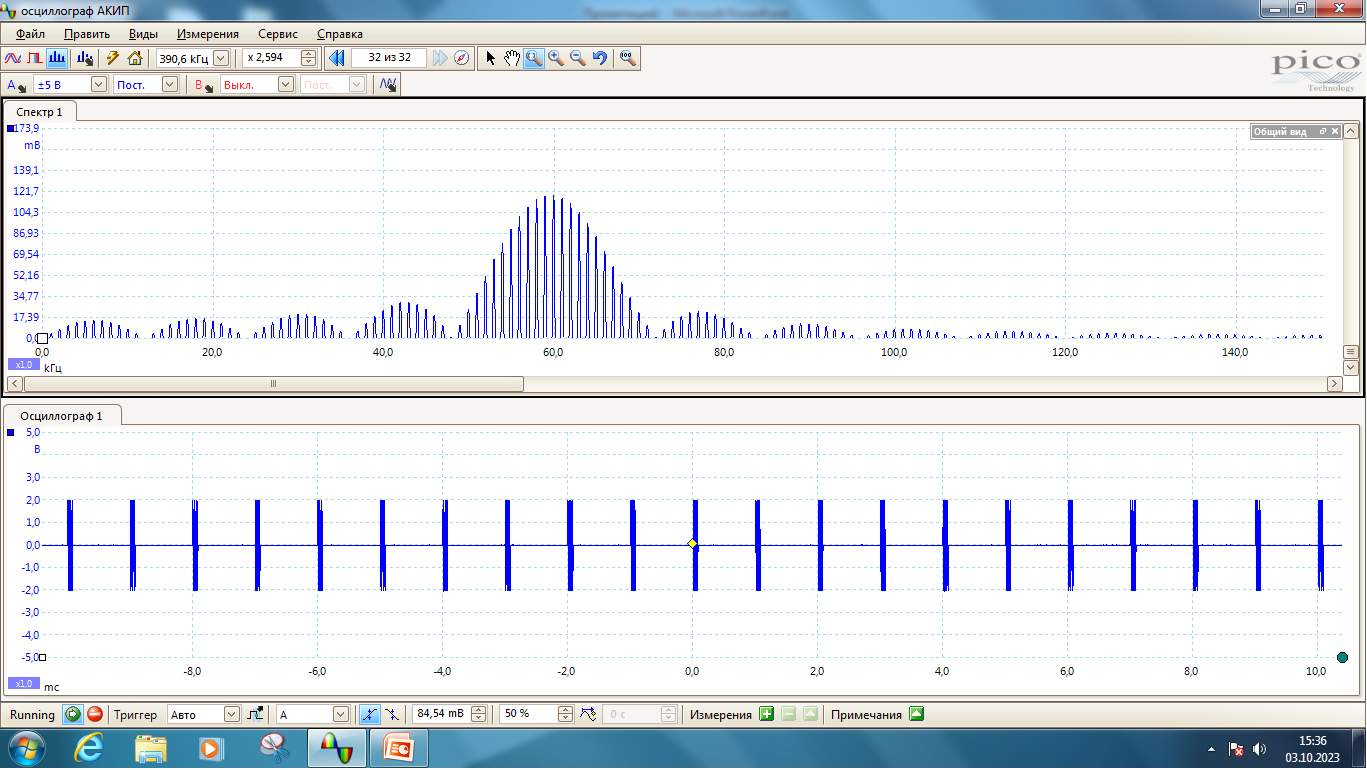
\includegraphics[width=0.5\textwidth]{images/spectrum_B_6.png}}} \\
        \subfloat[$\nu_0 = 70$ кГц, $T = 1$ мс, $N = 5$]{{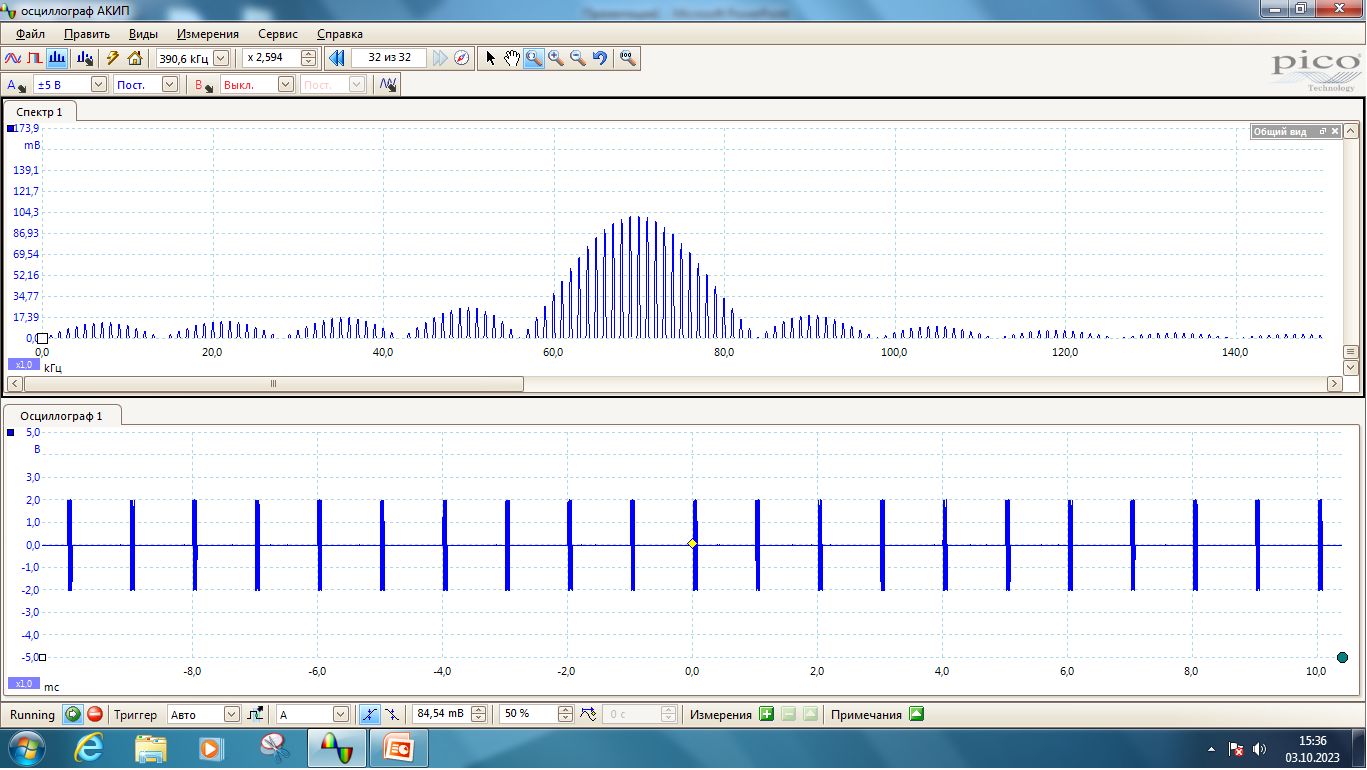
\includegraphics[width=0.5\textwidth]{images/spectrum_B_7.png}}}
        \caption{Изменение спектра синусоидальных импульсов при варьировании параметров}
        \label{spectrum_B}
    \end{figure}

    По данным таблицы \ref{table:zug} построим график зависимости $\delta \nu \left( 1/T \right)$ (рис. \ref{graph:zug}).

    \begin{figure}[H]
        \centering
        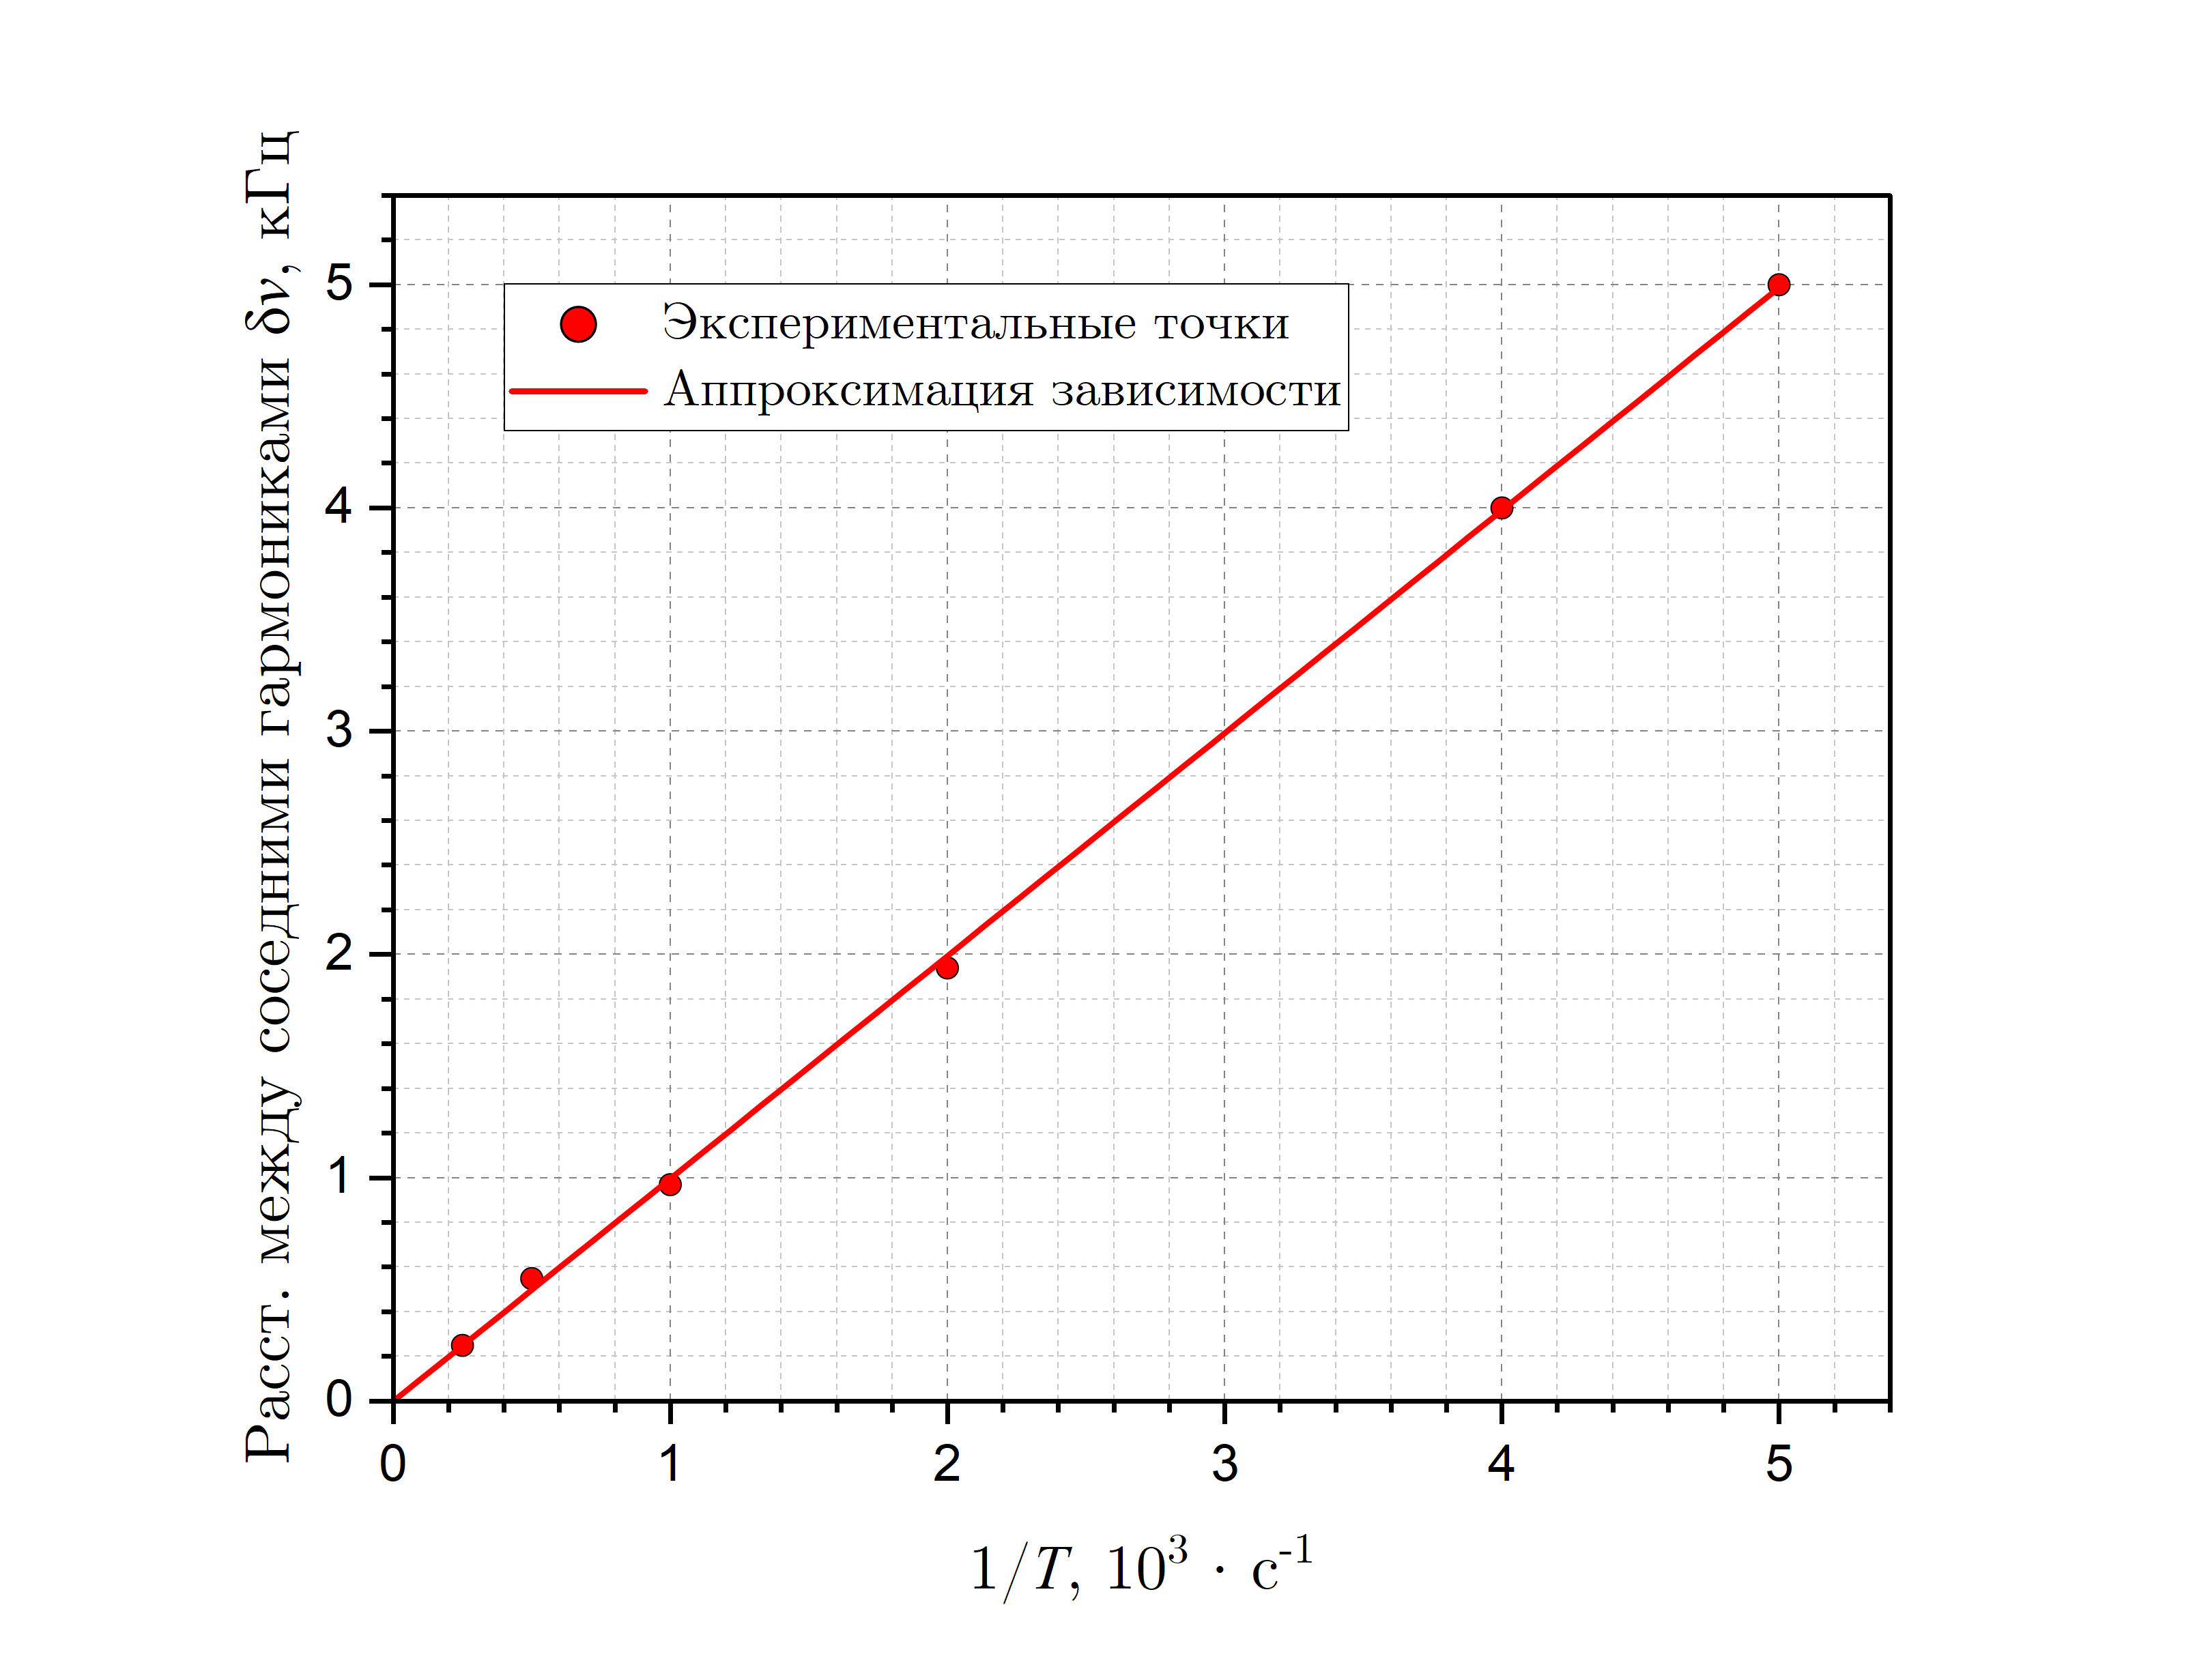
\includegraphics[width = 14 cm]{images/graph_zug.png}
        \caption{График зависимости расстояния между соседними гармониками $\delta \nu$ от $1/T$}
        \label{graph:zug}
    \end{figure}

    Аппроксимируя полученные данные при помощи программы \textit{OriginPro 2023b}, получим

    $$
    \boxed{\delta \nu \cdot T = 0,997 \pm 0,005}, 
    $$

    что согласуется с соотношением неопределённости (см. пункт \ref{theor_uncertainty}).

    \subsection{Исследование спектра амплитудно-модулированного сигнала}

    Установив на генераторе режим \textit{модулированного по амплитуде} синусоидального сигнала с несущей частотой $\nu_0 = 50$ кГц, частотой модуляции $\nu_\text{мод} = 2$ кГц и глубиной модуляции $50 \%$ ($m = 0,5$), получили на экране осциллографа устойчивую картину сигнала.

    Измерим максимальную $A_{max}$ и минимальную $A_{min}$ амплитуды сигнала, чтобы вычислить значение $m$, получим

    \begin{equation*}
         m = \frac{A_{max} - A_{min}}{A_{max} + A_{min}} = \frac{1,504 \text{ В} - 0,499 \text{ В}}{1,504 \text{ В} + 0,499 \text{ В}} \approx 0,5.
    \end{equation*}

    Полученное значение эквивалентно тому, что установлено на генераторе.

    Изменяя на генераторе несущую частоту $\nu_0$ и частоту модуляции $\nu_\text{мод}$, зафиксировали, как изменялось положение спектральных линий (рис. \ref{spectrum_C}).

    \begin{figure}[H]
        \centering
        \subfloat[$\nu_0 = 50$ кГц, $\nu_{\text{мод}} = 2$ кГц]{{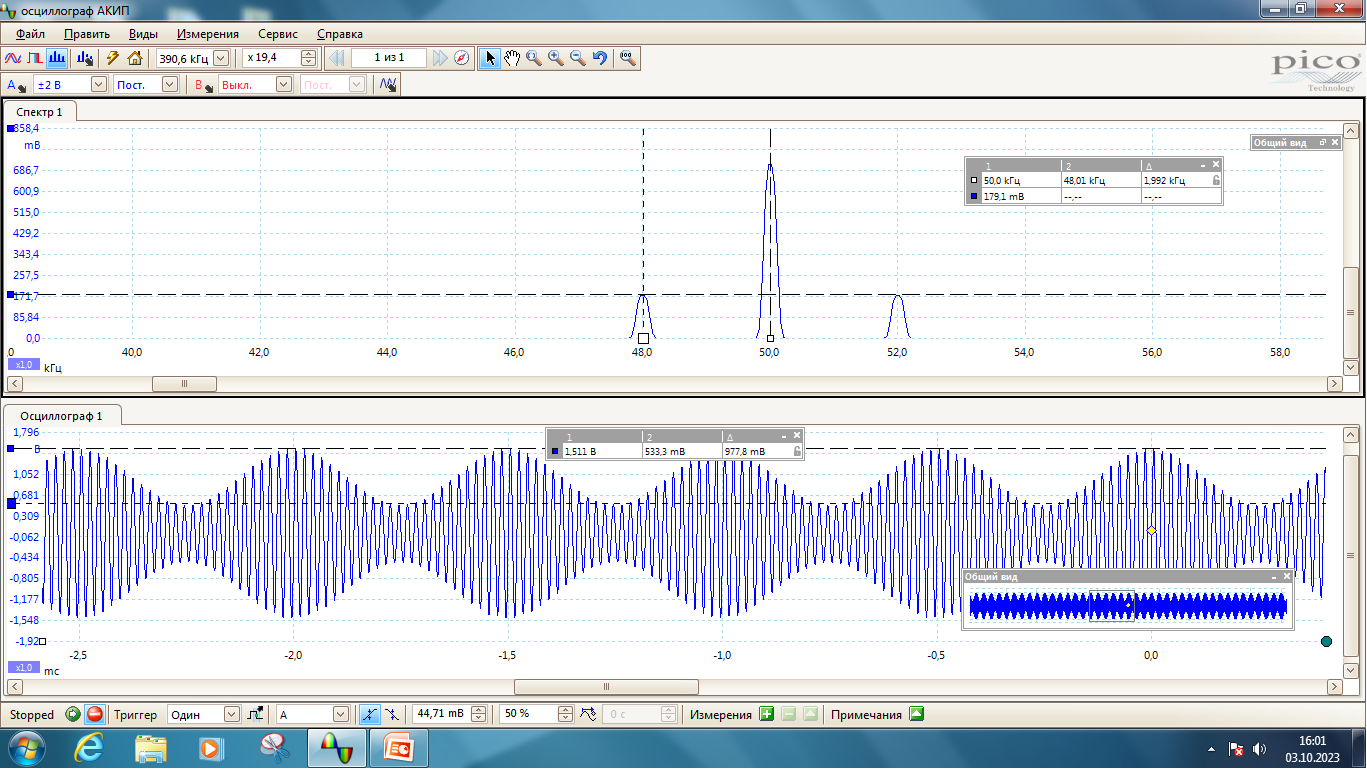
\includegraphics[width=0.5\textwidth]{images/spectrum_C_1.png}}}
        \subfloat[$\nu_0 = 60$ кГц, $\nu_{\text{мод}} = 2$ кГц]{{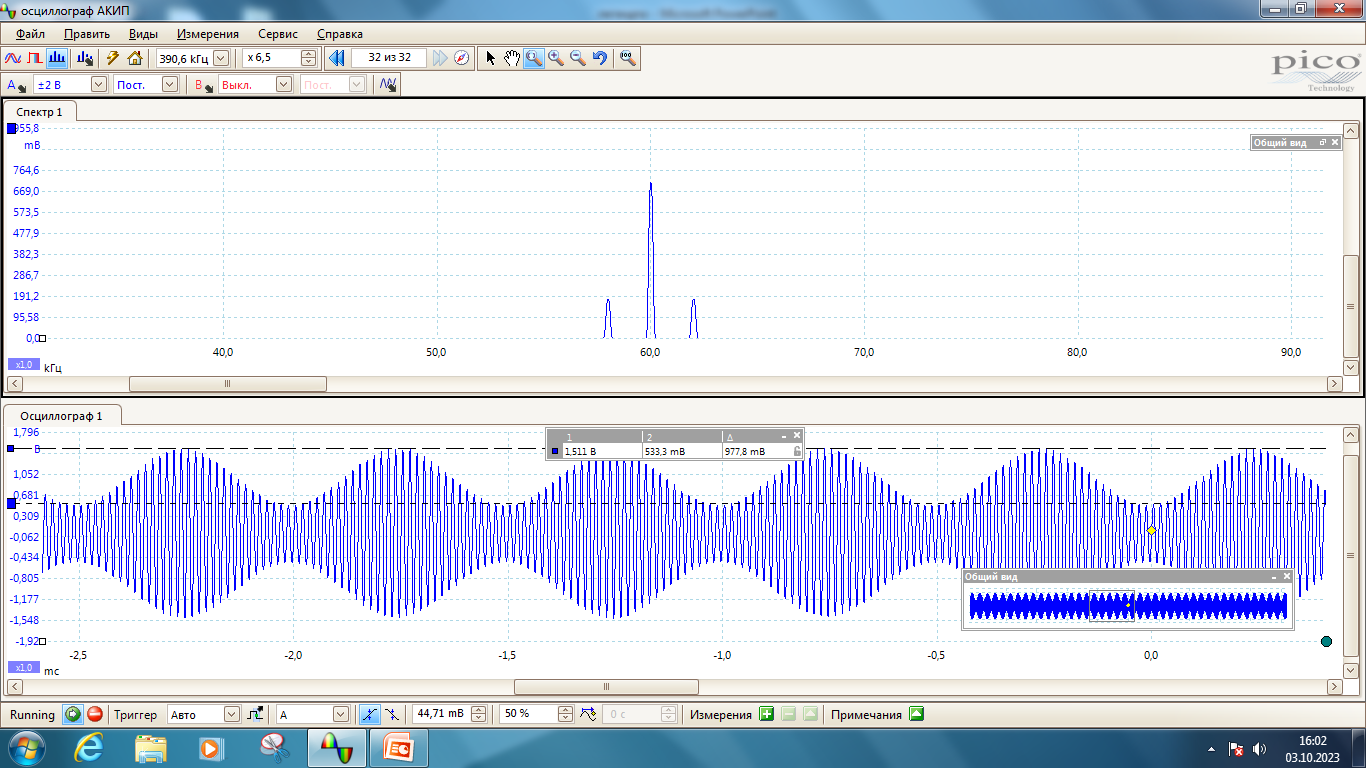
\includegraphics[width=0.5\textwidth]{images/spectrum_C_2.png}}}\\
        \subfloat[$\nu_0 = 40$ кГц, $\nu_{\text{мод}} = 2$ кГц]{{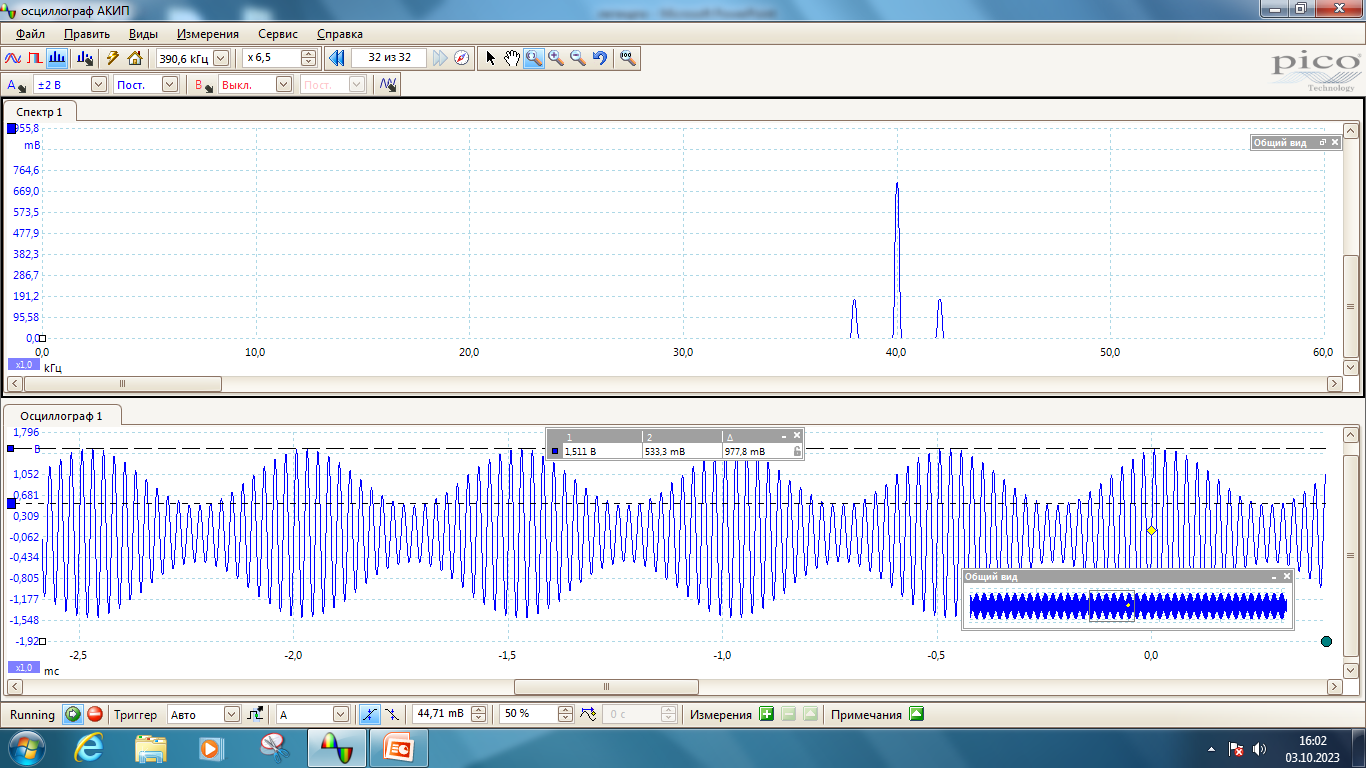
\includegraphics[width=0.5\textwidth]{images/spectrum_C_3.png}}}    		
        \subfloat[$\nu_0 = 50$ кГц, $\nu_{\text{мод}} = 4$ кГц]{{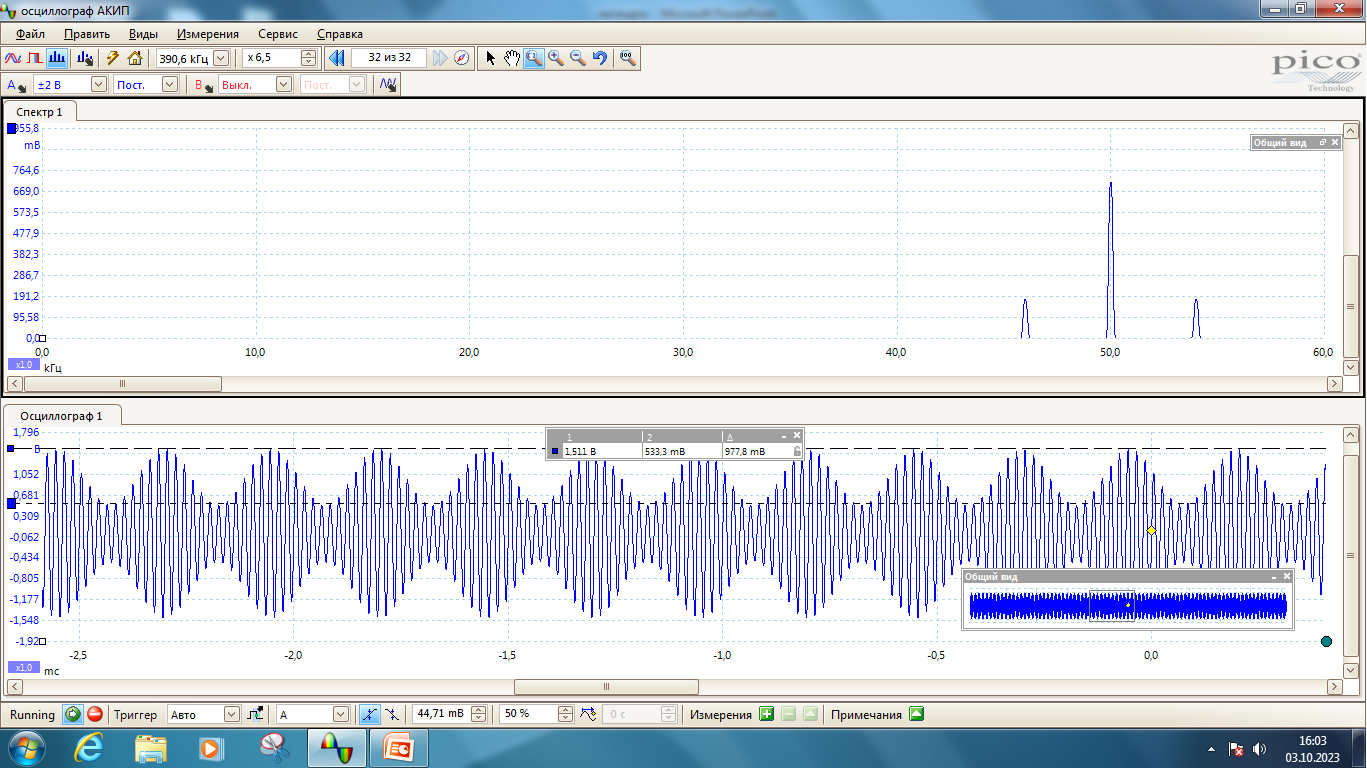
\includegraphics[width=0.5\textwidth]{images/spectrum_C_4.png}}}
        \caption{Изменение спектральных линий при варьировании параметров}
        \label{spectrum_C}
    \end{figure}

    Изменяя на генераторе глубину модуляции $m$, измерим отношение амплитуд боковой $a_\text{бок}$ и основной $a_\text{осн}$ спектральных линий. Полученные результаты приведены в таблице \ref{modulation}.

    \begin{table}[H]
        \centering
        \begin{tabular}{|c|c|c|c|}
        \hline
        $m$, \% & $a_\text{бок}$, В & $a_\text{осн}$, В & $a_\text{бок}/a_\text{осн}$ \\ \hline
        10 & 37,2 & \multirow{10}{*}{712,7} & 0,0522 \\ \cline{1-2} \cline{4-4} 
        20 & 70,2 &  & 0,0986 \\ \cline{1-2} \cline{4-4} 
        30 & 105,4 &  & 0,1479 \\ \cline{1-2} \cline{4-4} 
        40 & 142,5 &  & 0,1999 \\ \cline{1-2} \cline{4-4} 
        50 & 177,7 &  & 0,2493 \\ \cline{1-2} \cline{4-4} 
        60 & 212,8 &  & 0,2986 \\ \cline{1-2} \cline{4-4} 
        70 & 250,0 &  & 0,3508 \\ \cline{1-2} \cline{4-4} 
        80 & 285,1 &  & 0,4000 \\ \cline{1-2} \cline{4-4} 
        90 & 320,2 &  & 0,4493 \\ \cline{1-2} \cline{4-4} 
        100 & 356,4 &  & 0,5001 \\ \hline
        \end{tabular}
        \caption{Результаты измерения зависимости $a_\text{бок}/a_\text{осн}$ от $m$}
        \label{modulation}
    \end{table}

    По этим данным построим график зависимости отношения амплитуд $a_\text{бок}/a_\text{осн}$ от глубины модуляции $m$ (рис. \ref{graph:modulation}).

    \begin{figure}[H]
        \centering
        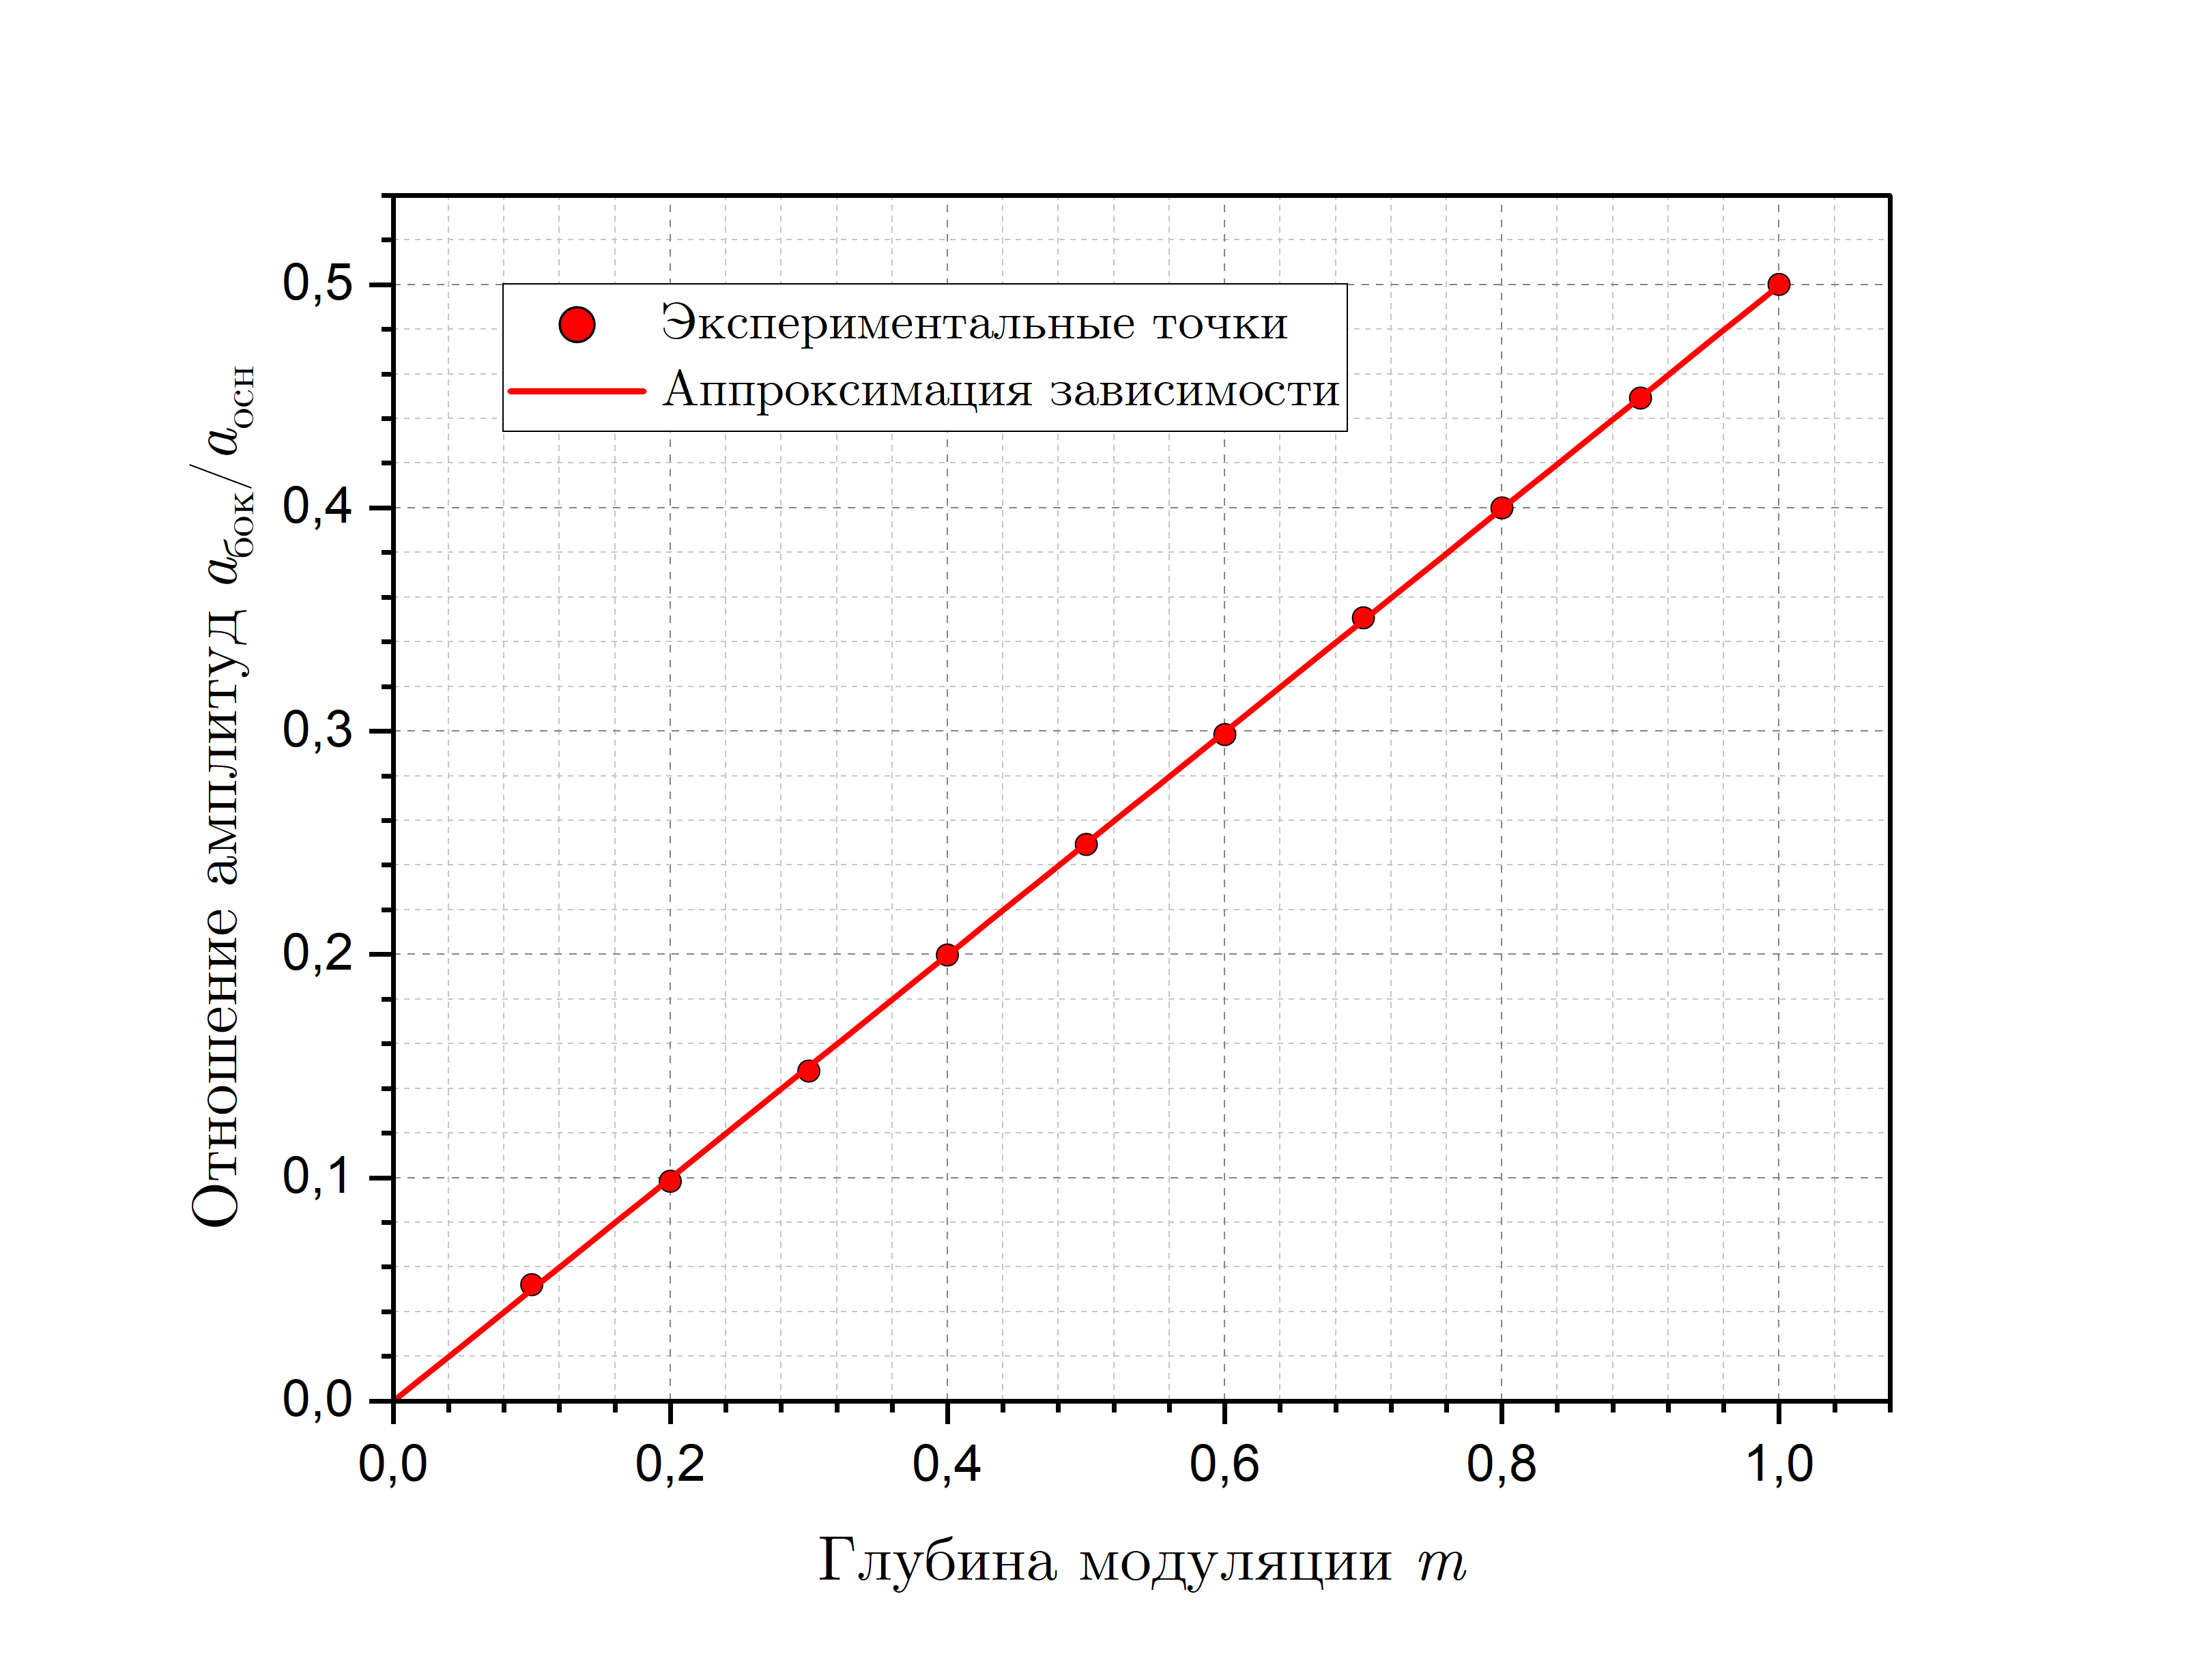
\includegraphics[width = 14 cm]{images/graph_modulation.png}
        \caption{График зависимости $a_\text{бок}/a_\text{осн}$ от $m$}
        \label{graph:modulation}
    \end{figure}

    Аппроксимируя полученные данные при помощи программы \textit{OriginPro 2023b}, получим, что коэффициент наклона графика равен

    \begin{equation*}
        k_{exp} = \left( 0,4995 \pm 0,0006 \right).
    \end{equation*}

    Полученное значение $k_{exp}$ эквивалентно теоретическому $k_{theor} = 0,5$ в пределах погрешности.

    \subsection{Изучение фильтрации сигналов}

    Собрав схему с \textit{RC}-фильтром низких частот с сопротивлением $R = 3$ кОм и ёмкостью $C = 10^{-9} \text{ Ф}$ ($\tau_{RC} = 3 \cdot 10^{-6}$ с, $\nu_{RC} = 333$ кГц), наблюдали форму сигнала и его спектр при различных значениях периода повторения $T$ (рис. \ref{spectrum_D}).

    Далее, при некотором фиксированном периоде $T$ провели измерения отношений амплитуд соответствующих спектральных гармоник фильтрованного и исходного сигналов: $K_n = \lvert a_n^{\phi} \rvert / \lvert a_n^{0} \rvert$. Результаты приведены в таблице \ref{table:K(nu)}.

    \begin{table}[H]
        \centering
        \begin{tabular}{|c|c|c|c|c|c|}
        \hline
        $n$ & $\nu_0$, кГц & $\nu$, кГц & $\lvert a_n^{\phi} \rvert$, мВ & $\lvert a_n^{0} \rvert$, мВ & $K_n = \lvert a_n^{\phi} \rvert / \lvert a_n^{0} \rvert$ \\ \hline
        1 & \multirow{8}{*}{35} & 35 & 233 & 286 & 0,8147 \\ \cline{1-1} \cline{3-6} 
        2 &  & 70 & 164 & 276 & 0,5942 \\ \cline{1-1} \cline{3-6} 
        3 &  & 105 & 120 & 270 & 0,4444 \\ \cline{1-1} \cline{3-6} 
        4 &  & 140 & 94 & 260 & 0,3615 \\ \cline{1-1} \cline{3-6} 
        5 &  & 175 & 70 & 253 & 0,2767 \\ \cline{1-1} \cline{3-6} 
        6 &  & 210 & 60 & 240 & 0,2500 \\ \cline{1-1} \cline{3-6} 
        7 &  & 245 & 48 & 225 & 0,2133 \\ \cline{1-1} \cline{3-6} 
        8 &  & 280 & 38 & 208 & 0,1827 \\ \hline
        \end{tabular}
        \caption{Результаты измерения зависимости $\lvert a_n^{\phi} \rvert / \lvert a_n^{0} \rvert$ от $\nu$}
        \label{table:K(nu)}
    \end{table}
    
    \begin{figure}[H]
        \centering
        \subfloat[$T = 3$ мкс, $\tau = 0,15$ мкс]{{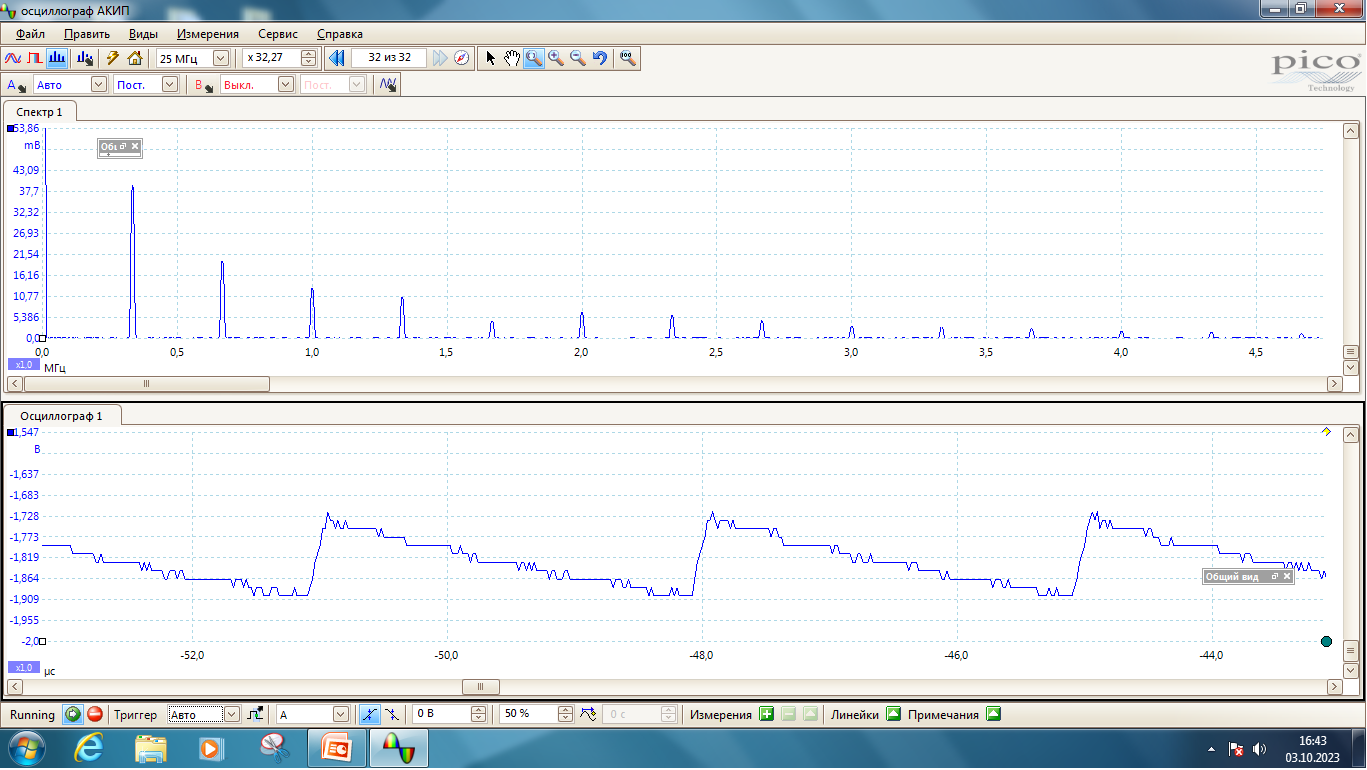
\includegraphics[width = 0.5\textwidth]{images/spectrum_D_1.png}}}
        \subfloat[$T = 2$ мкс, $\tau = 0,15$ мкс]{{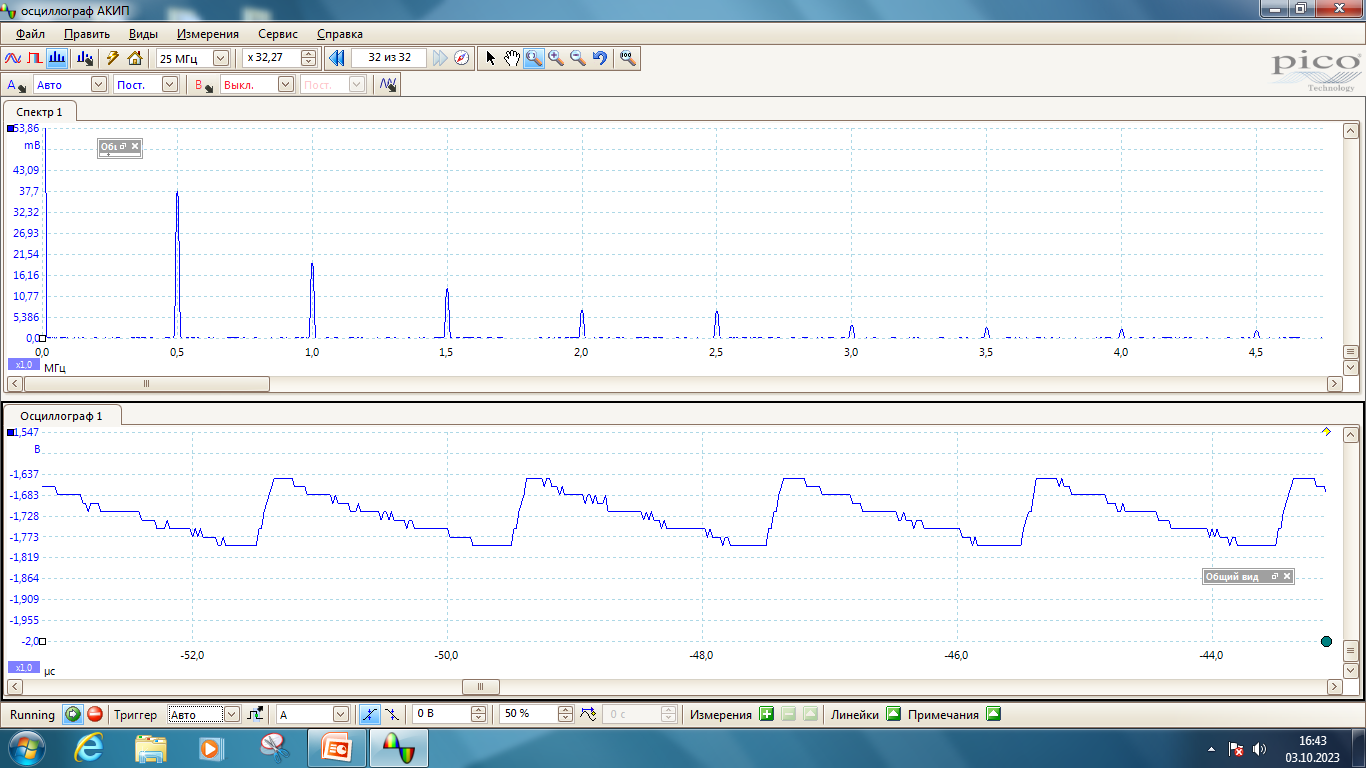
\includegraphics[width = 0.5\textwidth]{images/spectrum_D_2.png}}} \\
        \subfloat[$T = 1$ мкс, $\tau = 0,15$ мкс]{{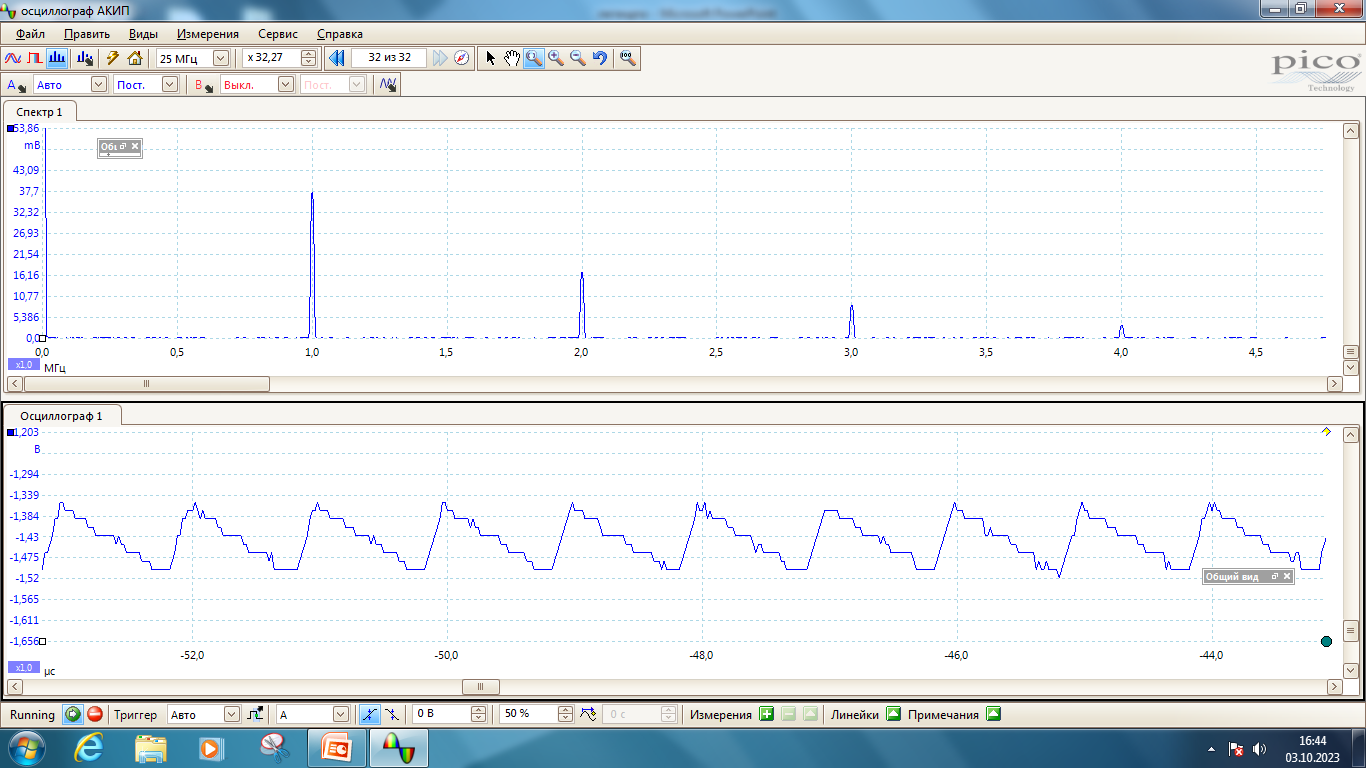
\includegraphics[width = 0.5\textwidth]{images/spectrum_D_3.png}}}
        \caption{Изменение спектра \textit{RC}-цепочки при варьировании $T$}
        \label{spectrum_D}
    \end{figure}

     По данным таблицы \ref{table:K(nu)} построим график зависимости $K(\nu)$ (рис. \ref{graph:K(nu)}).

    \begin{figure}[H]
        \centering
        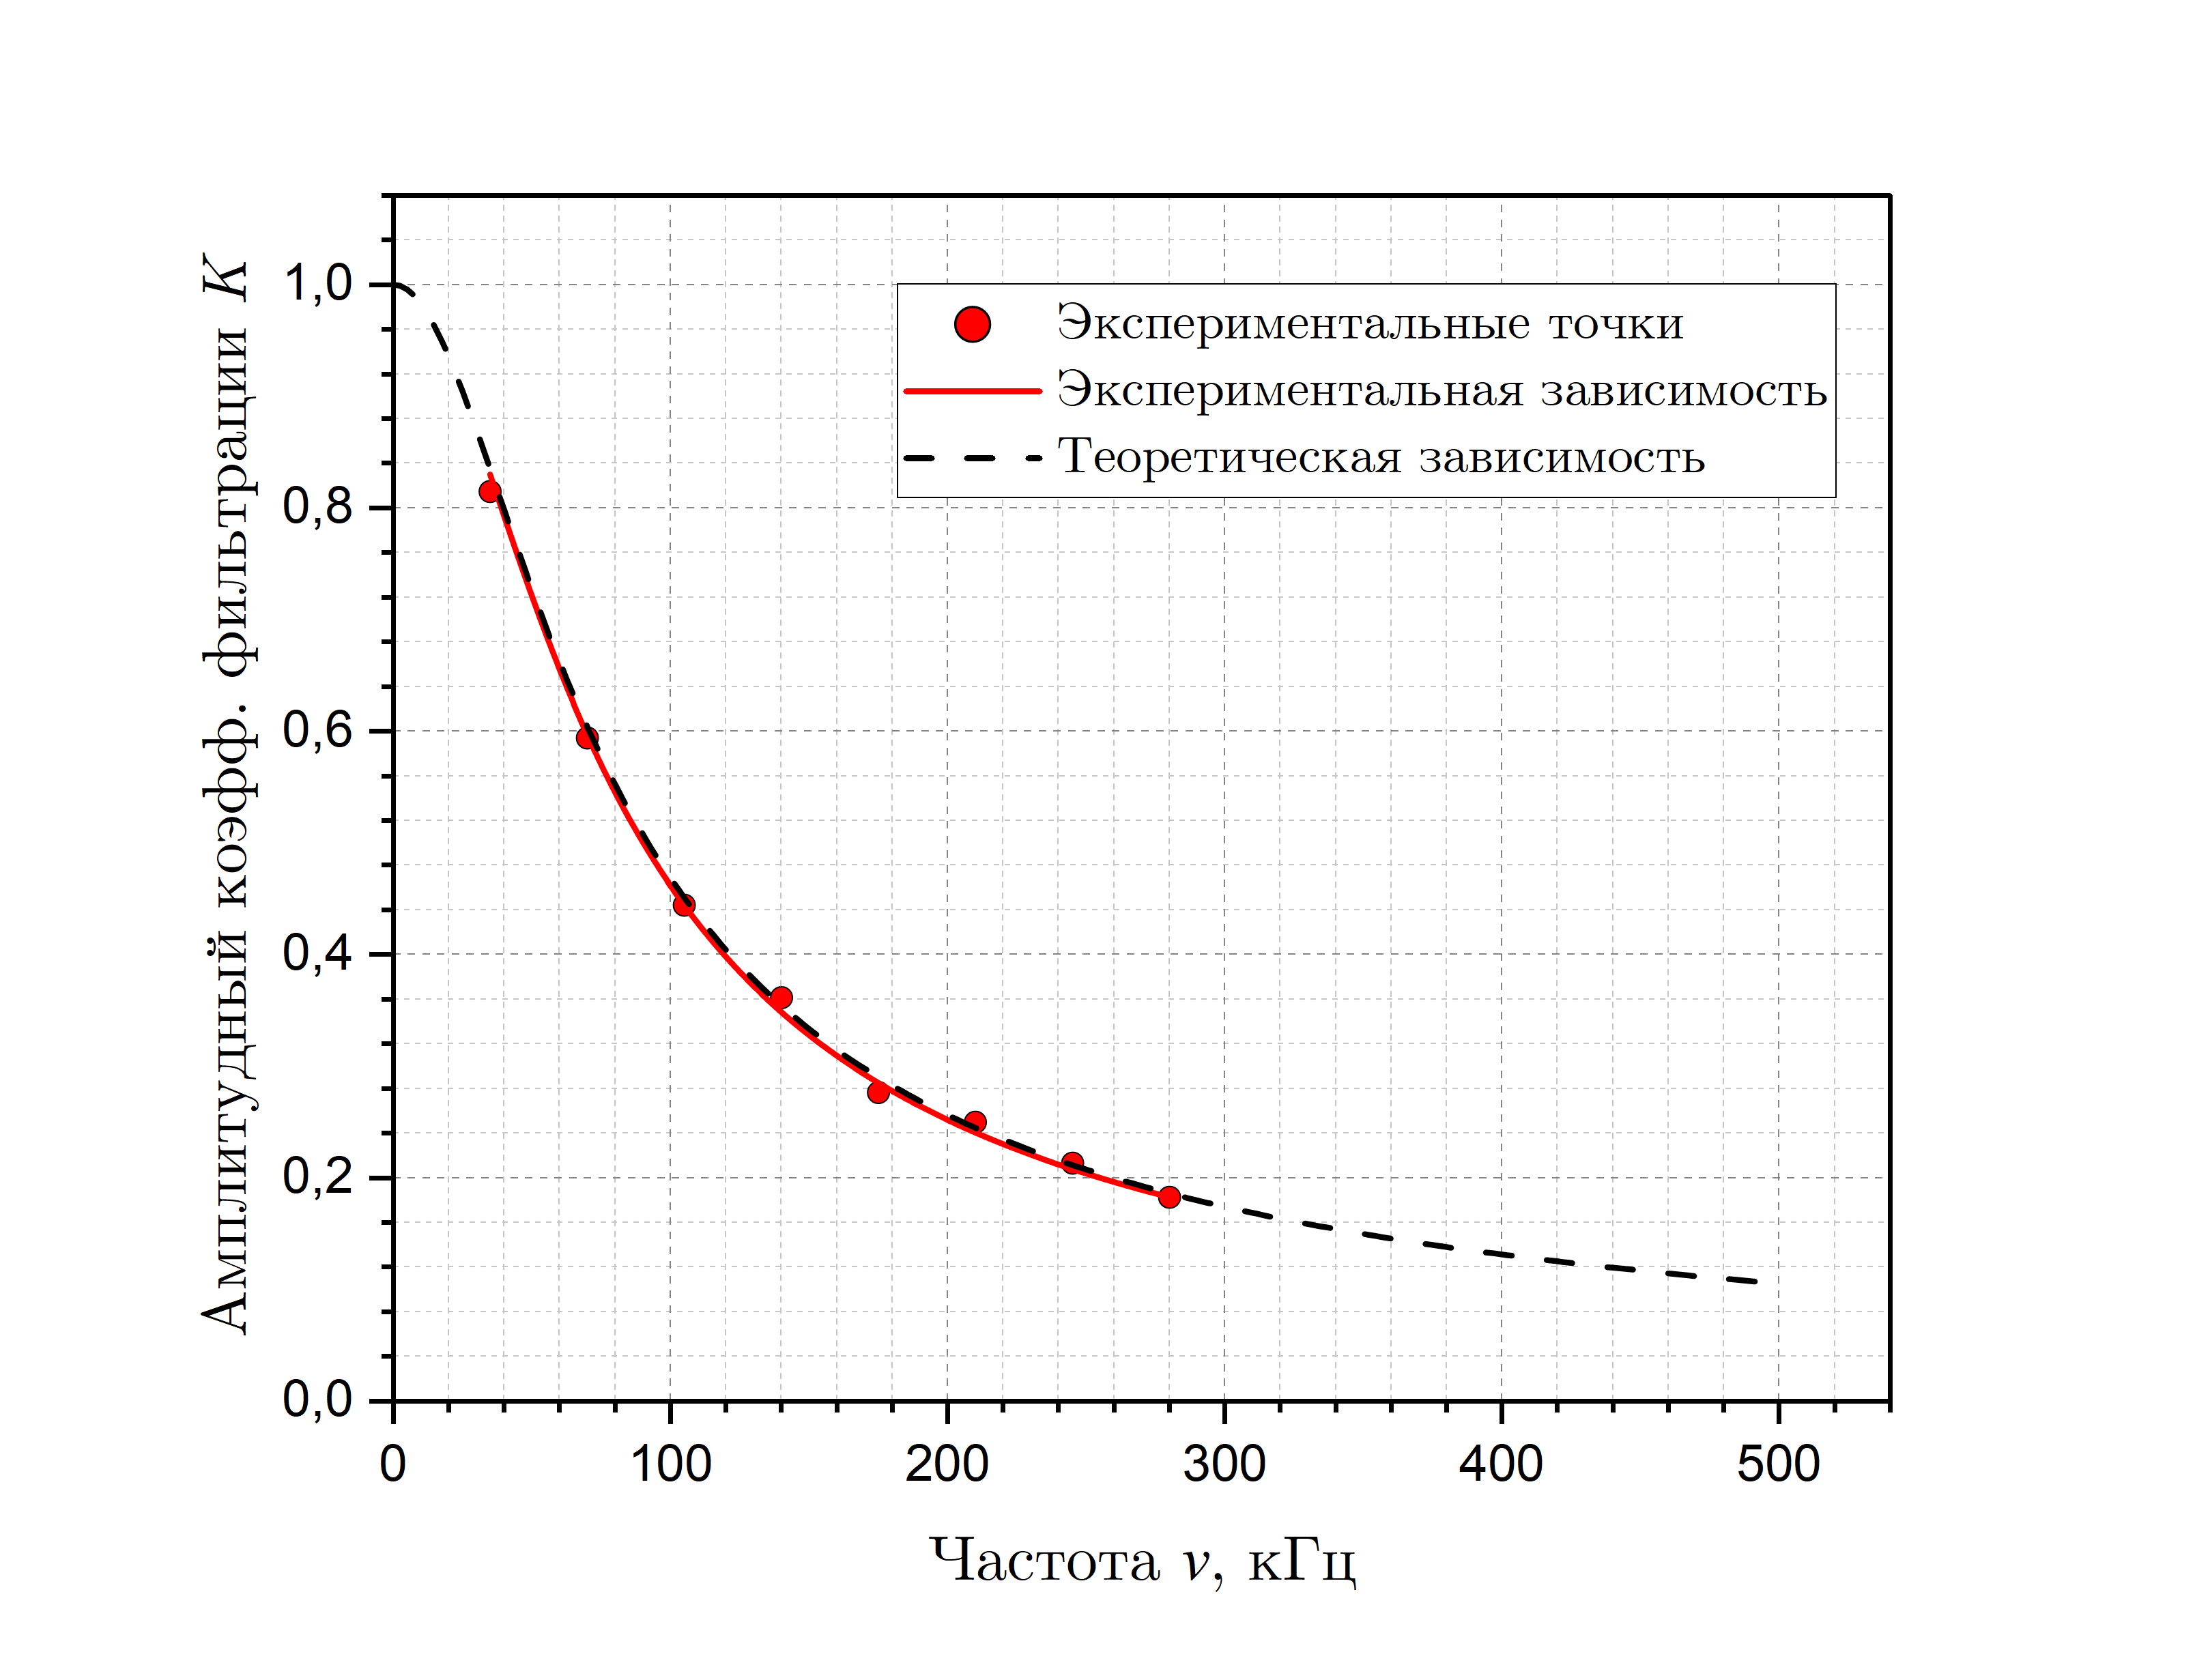
\includegraphics[width = 14 cm]{images/graph_K(nu).png}
        \caption{График зависимости амплитудного коэффициента фильтрации $K$ от частоты $\nu = n \nu_0$}
        \label{graph:K(nu)}
    \end{figure}

     Аппроксимируя полученные данные зависимостью вида $K(\nu) = 1/\sqrt{1 + 4 \pi^2 R^2 C^2 \nu^2}$ при помощи программы \textit{OriginPro 2023b}, получим, что

     \begin{equation*}
         4 \pi^2 R^2C^2 = \left( 3,7 \pm 0,1 \right) \cdot 10^{-10} \text{ c}^2 \Rightarrow \tau_{RC}^{exp} = \left( 3,05 \pm 0,05 \right) \cdot 10^{-6} \text{ с}.
     \end{equation*}

     Полученное значение $\tau_{RC}^{exp}$ совпадает с $\tau_{RC}^{theor} = 3 \cdot 10^{-6}$ с в пределах погрешности.

    \section{Заключение}

    В данной работе были изучены спектры периодических электрических сигналов.
    
    В первой части работы было проверено и экспериментально подтверждено соотношение неопределённостей $\Delta\nu \cdot \tau = 1$ для прямоугольных импульсов.

    Во второй части работы были исследованы спектры цугов гармонических колебаний, экспериментально подтвержджён тот факт, что при стремлении частоты повторения цугов к нулю спектр переходит в непрерывный.

    В последней части работы были исследованы спектры гармонических сигналов, модулированных по амплитуде. Экспериментально подтверждено соотношение $\frac{a_{\text{бок}}}{a_{\text{осн}}}=\frac{m}{2}$.

    Результаты оценки погрешностей говорят о хорошей точности использованных методов и корректном проведении эксперимента.

\end{document}